\documentclass[oneside,a4paper,11pt]{book}
\usepackage[utf8]{inputenc}
\usepackage{svg}
\usepackage[italian]{babel}
\usepackage{float}
\usepackage{fancyvrb}
\usepackage{titling}
\usepackage[margin=1in,footskip=0.25in]{geometry}
\usepackage{listings}
\usepackage[DIV=12,BCOR=2mm,headinclude=true,footinclude=false]{typearea}
\usepackage{color, colortbl,xcolor}
\usepackage[hidelinks]{hyperref}
\usepackage{tcolorbox}
\usepackage{chngcntr}
\usepackage{diagbox}
\usepackage{calc}
\usepackage{amssymb}
\usepackage{subcaption}
\usepackage{amsthm}
\usepackage{amsfonts}
\usepackage{mathtools}
\usepackage{parskip}
\usepackage{cancel}
\usepackage{forest}
\usepackage{listings}
\usepackage{mathrsfs}
\usepackage{enumitem}
\usepackage{makecell}
\usepackage{tikz}
\usepackage{pgfplots}
\pgfplotsset{compat=1.18}
\usepackage{fancyhdr}
\fancypagestyle{plain}{\fancyhf{}\renewcommand{\headrulewidth}{0pt}}
\pagestyle{fancy}
\fancyhf{}% Clear header/footer
\fancyhead[L]{\nouppercase\leftmark}
\fancyhead[R]{\thepage}
\usetikzlibrary{positioning,shapes.geometric,arrows.meta,matrix,automata,decorations.pathmorphing,patterns,
decorations.pathreplacing,shapes.multipart,calc,snakes}
\usetikzlibrary{arrows.meta, backgrounds, chains, positioning, shapes.geometric, shapes.multipart, graphs, graphs.standard}

\tcbuselibrary{skins}
\counterwithin{figure}{section}
%Nuovi comandi
\newcommand\myeq{\stackrel{\mathclap{\normalfont\mbox{def}}}{=}}
\newcommand\prodG{\stackrel{\mathclap{\normalfont\mbox{\tiny{G}}}}{\Longrightarrow}}

\usepackage{syntax}
\usepackage[linesnumbered,ruled,vlined]{algorithm2e}
% Definizione di uno stile personalizzato per la grammatica
\setlength{\grammarparsep}{20pt plus 1pt minus 1pt} % increase separation between rules
\setlength{\grammarindent}{12em} % increase separation between LHS/RHS 
% Rimuovi le parentesi angolari attorno al nome delle produzioni
\renewcommand{\grammarlabel}[2]{\textit{#1}\ \ #2\ \ }

\newcommand{\llbracket}{[\![}
\newcommand{\rrbracket}{]\!]}

%asmthm
\newlength{\marginlabelsep}\setlength{\marginlabelsep}{0.5em}
\newtheoremstyle{italicstyle} %% Name
  {} %% <- Space above (empty = default = \topsep = 8.0pt plus 2.0pt minus 4.0pt)
  {} %% <- Space below (empty = default = \topsep = 8.0pt plus 2.0pt minus 4.0pt)
  {\itshape} %% <- Body font
  {} %% <- Indent amount (empty = no indent, \parindent = just that)
  {\bfseries} %% <- Thm head font
  {} %% <- Punctuation after thm head
  {1pt} %% <- Space after thm head (or " " or \newline) (default: 5pt plus 1pt minus 1pt)
  {\vtop to 0pt{\llap{\thmname{#1}\hskip\marginlabelsep}
                \llap{\thmnumber{#2}\hskip\marginlabelsep}}\thmnote{#3\\}%
  }
\newtheoremstyle{normStyle} %% Name
  {} %% <- Space above (empty = default = \topsep = 8.0pt plus 2.0pt minus 4.0pt)
  {} %% <- Space below (empty = default = \topsep = 8.0pt plus 2.0pt minus 4.0pt)
  {\normalfont} %% <- Body font
  {} %% <- Indent amount (empty = no indent, \parindent = just that)
  {\bfseries} %% <- Thm head font
  {} %% <- Punctuation after thm head
  {1pt} %% <- Space after thm head (or " " or \newline) (default: 5pt plus 1pt minus 1pt)
  {\vtop to 0pt{\llap{\thmname{#1}\hskip\marginlabelsep}
                \llap{\thmnumber{#2}\hskip\marginlabelsep}}\thmnote{#3\\}%
  }
\theoremstyle{italicstyle}
\newtheorem{corollary}{Corollario}[section]
\newtheorem{notazione}{Notazione}[section]
\newtheorem{lemma}{Lemma}[section]
\newtheorem{definizione}{Definizione}[section]
\newtheorem{nota}{Nota}[section]
\newtheorem{exercise}{Esercizio}[section]
\theoremstyle{normStyle}
\newtheorem{exmp}{Esempio}[section]
\newtheorem{theorem}{Teorema}[section]
\newtheorem{proposizione}{Proposizione}[section]
\tcbuselibrary{listings,skins}
\newtcblisting{mylisting}[2][]{
    arc=0pt, outer arc=0pt,
    listing only, 
    title=#2,
    #1,
    listing options= {escapechar=|}
}

\newcommand{\mybox}[3]{
  \begin{tcolorbox}[colback=#2!10, colbacktitle=#2!30!black, colframe=black, title=#1]
    #3
    \ignorespaces
  \end{tcolorbox}
}
\newcommand{\myboxedtext}[2][rectangle,draw]{%
    \tikz[baseline=-0.6ex] \node [#1]{#2};}%

\usetikzlibrary{decorations.pathreplacing,calligraphy}
%%======================================================================
\title{Analisi del Software}
\author{\textit{Alessio Gjergji}}
\date{}
\begin{document}
\maketitle
\tableofcontents
\chapter{Introduzione}
\section{Linguaggi di programmazione}
Un linguaggio di programmazione è un linguaggio formale che specifica un
insieme di istruzioni che possono essere usate per produrre un insieme di
output.
Esso è definito da:
\begin{itemize}
    \item \textbf{Sintassi}: specifica la forma delle istruzioni. Ci permette di
    capire quali stringhe sono ammissibili e quali no mediante diversi strumenti come 
    grammatiche, analizzatori lessicali e sintattici, teoria degli automi.
    \item \textbf{Pragmatica}: specifica l'effetto delle istruzioni. Ci permette
    di capire le ragioni per introdurre un nuovo linguaggio e di programmazione 
    invece di utilizzarne uno già esistente.
    \item \textbf{Semantica}: specifica il significato dei programmi scritti nel linguaggio, ovvero il loro 
    comportamento a tempo di esecuzione. Ci permette di capire se due programmi 
    apparentemente diversi sono equivalenti.
\end{itemize}
\subsection{Benefici di una semantica formale}
I benefici dei linguaggi di programmazione diversi, tra cui:
\begin{itemize}
    \item \textbf{Implementazione}: Consente di fornire la specifica (\textit{del comportamento}) 
    dei programmi indipendentemente dalla macchina o dal compilatore utilizzato.
    \item \textbf{Verifica}: una semantica formale consente di ragionare 
    sui programmi e sulle loro proprietà di correttezza.
    \item \textbf{Progettazione di Linguaggio}: spesso una semantica formale consente di 
    scoprire ambiguità all'interno di linguaggi già esistenti. Questo aiuta a progettare 
    nuovi linguaggi in maniera più accurata.
\end{itemize}
\section{Un linguaggio per le espressioni aritmetiche: sintassi}
Definiamo il seguente linguaggio:
\[
    \mathcal{E}\quad ::= \quad n \quad | \quad \mathcal{E} + \mathcal{E} \quad | 
    \quad \mathcal{E} * \mathcal{E} \quad | \quad \dots
\]
dove:
\begin{itemize}
    \item $n$ è lo spazio del dominio dei numerali.
    \item $\mathcal{E}$ è il range del dominio delle espressioni aritmetiche.
    \item $+, x, \dots$ sono simboli del linguaggio.
\end{itemize}
I numerali sono parte della sintassi del nostro linguaggio e non vanno confusi con i numeri
che sono oggetti matematici.
Ciò potrebbe significare che nel nostro linguaggio al posto di $0, 1, \dots$ avremmo 
potuto usare $zero, uno, \dots$ e sarebbero potuti essere uguali.

Nel nostro caso assumiamo che esista una corrispondenza ovvia tra il simbolo ``numerale" (n)
e il numero naturale n. Questo è fatto solo per semplificare la spiegazione. In un
altro contesto, il simbolo ``numeral" 3 potrebbe essere associato al numero 42!

\section{Semantica Operazionale}

La semantica operazionale ha l'obiettivo di valutare un'espressione aritmetica
del linguaggio per ottenere il suo valore numerico associato. Questo può essere
fatto in due modi differenti:

\begin{itemize}
  \item \textbf{Semantica Small-Step (\textit{o strutturale})}: Fornisce un metodo per
  valutare un'espressione passo dopo passo, considerando le azioni intermedie.
  Questo approccio fornisce una valutazione dettagliata dell'espressione.

  \item \textbf{Semantica Big-Step (\textit{o naturale})}: Ignora i passaggi intermedi
  e fornisce direttamente il risultato finale della valutazione dell'espressione. Questo
  approccio semplifica la valutazione, concentrando l'attenzione sul risultato finale.

\end{itemize}
\subsection{Big-Step Semantics}

\begin{tcolorbox}[title = {Valutazione}]  
    $E \Downarrow n$
\end{tcolorbox}
\textbf{Significato}: La valutazione dell'espressione $\mathcal{E}$ produce il numerale $n$.

\begin{tcolorbox}[title = {Assiomi e regole di inferenza}]  
\begin{figure}[H]
    \begin{subfigure}{0.3\textwidth}
    \begin{prooftree}
        \AxiomC{$-$}
        \LeftLabel{(B-Num)}
        \UnaryInfC{$n \Downarrow n$}
    \end{prooftree}
    \end{subfigure}%
    \begin{subfigure}{0.7\textwidth}
    \begin{prooftree}
        \AxiomC{$\mathcal{E}_1 \Downarrow n_1$}
        \AxiomC{$\mathcal{E}_2 \Downarrow n_2$}
        \LeftLabel{(B-Add)}
        \RightLabel{$n_3 = add(n_1, n_2)$}
        \BinaryInfC{$\mathcal{E}_1 + \mathcal{E}_2 \Downarrow n_3$}
    \end{prooftree}
    \end{subfigure}
\end{figure}
\end{tcolorbox}
\textbf{Significato}: 
\begin{itemize}
\item (B-Num): Questo è un assioma che afferma che quando valutiamo un singolo
numero $n$, otteniamo lo stesso numero $n$ come risultato. Questo è il caso
base della valutazione.

\item (B-Add): Questa regola di inferenza afferma che date due espressioni
$\mathcal{E}_1$ e $\mathcal{E}_2$:
\begin{itemize}
  \item Se è il caso che $\mathcal{E}_1 \Downarrow n_1$ (cioè $\mathcal{E}_1$ si valuta a $n_1$) e
  \item È anche il caso che $\mathcal{E}_2 \Downarrow n_2$ (cioè $\mathcal{E}_2$ si valuta a $n_2$),
  allora segue che $\mathcal{E}_1 + \mathcal{E}_2 \Downarrow n_3$, dove $n_3$ è il numerale associato
  al numero $n_3$ tale che $n_3 = add(n_1, n_2)$.
  Si noti che in questa regola, $E1$, $E2$, $n1$, $n2$, $n3$ sono meta-variabili.
\end{itemize}
\end{itemize}
Questa regola (B-Add) ci dice come valutare un'addizione tra due espressioni
$\mathcal{E}_1$ e $\mathcal{E}_2$ nel contesto della semantica big-step. La
regola stabilisce che se possiamo valutare entrambe le espressioni operandi
($\mathcal{E}_1$ e $\mathcal{E}_2$) e otteniamo i numeri $n_1$ e $n_2$ rispettivamente,
allora possiamo calcolare la somma di $\mathcal{E}_1$ e $\mathcal{E}_2$ come $n_3$,
dove $n_3$ è il risultato della somma dei numeri $n_1$ e $n_2$.
Si noti che la funzione di addizione $add$ opera sui numeri, non sui numerali.
\subsection{Small-Step Semantics}

\begin{tcolorbox}[title = {Valutazione}]  
$\mathcal{E}_1 \rightarrow \mathcal{E}_2$

\end{tcolorbox}
\textbf{Significato:} 
Dopo aver eseguito un passo di valutazione su $\mathcal{E}_1$, l'espressione $\mathcal{E}_2$ rimane da valutare.
\begin{tcolorbox}[title = {Assiomi e regole di inferenza}]  
\begin{prooftree}
    \AxiomC{$\mathcal{E}_1 \rightarrow \mathcal{E}_1'$}
    \LeftLabel{(S-Left)}
    \UnaryInfC{$\mathcal{E}_1 + \mathcal{E}_2 \rightarrow \mathcal{E}_1' + \mathcal{E}_2$}
    \end{prooftree}
    
    \begin{prooftree}
    \AxiomC{$\mathcal{E}_2 \rightarrow \mathcal{E}_2'$}
    \LeftLabel{(S-N.Right)}
    \UnaryInfC{$n_1 + \mathcal{E}_2 \rightarrow n_1 + \mathcal{E}_2'$}
    \end{prooftree}
    
    \begin{prooftree}
    \AxiomC{-}
    \LeftLabel{(S-Add)}
    \RightLabel{$n_3 = add(n_1, n_2)$}
    \UnaryInfC{$n_1 + n_2 \rightarrow n_3$}
    \RightLabel{(S-Add)}
\end{prooftree}
\end{tcolorbox}
Fissiamo l'ordine di valutazione da sinistra a destra. Qualcosa di 
simile non è possibile nella big-step semantics, dove le espressioni sono 
valutate in un solo passo.
\subsubsection{La scelta dell'ordine di valutazione}
\begin{tcolorbox}[title = {Assiomi e regole di inferenza}]  
    \begin{prooftree}
        \AxiomC{$\mathcal{E}_1 \rightarrow_{ch} \mathcal{E}_1'$}
        \LeftLabel{(S-Left)}
        \UnaryInfC{$\mathcal{E}_1 + \mathcal{E}_2 \rightarrow_{ch} \mathcal{E}_1' + \mathcal{E}_2$}
        \end{prooftree}
        
        \begin{prooftree}
        \AxiomC{$\mathcal{E}_2 \rightarrow_{ch} \mathcal{E}_2'$}
        \LeftLabel{(S-Right)}
        \UnaryInfC{$\mathcal{E}_1 + \mathcal{E}_2 \rightarrow_{ch} \mathcal{E}_1 + \mathcal{E}_2'$}
        \end{prooftree}
        
        \begin{prooftree}
        \AxiomC{-}
        \LeftLabel{(S-Add)}
        \RightLabel{$n_3 = add(n_1, n_2)$}
        \UnaryInfC{$n_1 + n_2 \rightarrow_{ch} n_3$}
        \RightLabel{(S-Add)}
    \end{prooftree}
\end{tcolorbox}
In questo caso non abbiamo precedenza stabilita per la valutazione delle espressioni.
Regole simili possono essere applicate anche con gli altri operatori.
\subsubsection{Esecuzione della small-step semantics}
La relazione $\rightarrow^k$, per $k \in \mathbb{N}$ è definita per un numero di passi 
di valutazione definito da $k$.
Mentre la relazione $\rightarrow^*$ è definita per un numero non definito di passi di valutazione.
\chapter{Modelliamo programmi}
\section{Un semplice linguaggio imperativo \texttt{IMP}}
Definiamo il linguaggio $\mathcal{L}$ dove:
\[
\begin{split}
    \mathbb{V} &= \mathbb{Z} \\
    \mathbb{X} &= \texttt{Var} \\
\end{split}
\]
\begin{grammar}
    <Exp $\mathbb{E}$> ::= $n\in \mathbb{V}$ | $x \in \mathbb{X}$ | 
    $\mathbb{E}  \oplus \mathbb{E}$

    <Bool $\mathbb{B}$> ::= \texttt{true} | \texttt{false} | $\mathbb{E} \oplus \mathbb{E}$

    <Com $\mathbb{C}$> ::= \texttt{skip} | $\mathbb{X} := \mathbb{E}$ | $\mathbb{C};\mathbb{C}$ |
    \texttt{if} $\mathbb{B}$ \texttt{then} $\mathbb{C}$ \texttt{else} $\mathbb{C}$
    \alt \texttt{while}  $\mathbb{B}$ | \texttt{input(x)} 

    <Programma $\mathbb{P}$> ::= $\mathbb{C}$
\end{grammar}
\subsection{La semantica di \texttt{IMP}}
La semantica è uno strumento formale che permette di dare significato ai programmi.


\begin{tcolorbox}[title = {Semantica operazionale}]
  La semantica operazionale è uno strumento formale che fornisce
  significato ai programmi attraverso la descrizione del comportamento
  passo dopo passo dell'interprete. Questo significa che il significato
  di un programma è descritto
  dalla sequenza dei singoli passi di computazione che esso compie.
\end{tcolorbox}

\begin{tcolorbox}[title = {Semantica denotazionale}]
  La semantica denotazionale attribuisce significato ai programmi
  tramite una funzione che associa a ciascun programma un valore.
  In termini matematici, possiamo rappresentare questa idea come segue:
    \[
      \texttt{intput}  \xrightarrow[\text{semantica}]{} \texttt{output} 
    \]
  In altre parole, esiste una funzione $\llbracket . \rrbracket$ che
  mappa l'input del programma all'output. Questa approccio è composito,
  il che significa che possiamo definire il significato di programmi
  composti in termini dei loro componenti, come segue:
    \[
      \llbracket . \rrbracket   : \texttt{intput}  \rightarrow \texttt{output}
    \]
    \[
      \llbracket P_1; P_2\rrbracket  = \llbracket P_2\rrbracket  \oplus \llbracket P_1\rrbracket
    \]
\end{tcolorbox}
Queste due forme di semantica, operazionale e denotazionale, sono
strumenti utili per comprendere
il significato dei programmi in modo dettagliato e matematico.
\subsection{Lo stato della memoria}
Nel contesto della programmazione, lo ``stato" rappresenta una
fotografia istantanea della configurazione della macchina (\textit{astratta})
su cui viene eseguito un programma. Questo stato descrive l'associazione
tra le variabili del programma e i valori che contengono. Formalmente,
possiamo rappresentare lo stato come una funzione $\mathbb{M}$ che
mappa le variabili ($\mathbb{X}$) ai loro valori ($\mathbb{V}$), come
segue:
\[
  \mathbb{M} : \mathbb{X} \rightarrow \mathbb{V}
\]
Durante l'esecuzione di un programma, viene generata una sequenza di
stati che riflettono come il programma modifica lo stato della memoria
nel corso del tempo. Questa sequenza di stati è essenziale per
comprendere come il programma funziona e come influisce sullo stato
della macchina. Nel contesto della modellazione formale, spesso ci
riferiamo a questo processo come ``esecuzione".

Per descrivere l'evoluzione di uno stato durante l'esecuzione di
un programma, utilizziamo un modello chiamato ``sistema di transizione",
che è rappresentato da una coppia $\langle \Sigma, \rightarrow \rangle$.
In questa coppia, $\Sigma$ rappresenta l'insieme degli stati possibili
e $\rightarrow$ rappresenta la relazione che specifica come un
determinato stato può transizionare in un altro stato a seguito
dell'esecuzione di un'azione del programma. Questo modello è
fondamentale per analizzare il comportamento dinamico di un programma
e comprendere come le modifiche di stato si verificano nel corso
dell'esecuzione.
\subsection{Semantica delle transizioni di stato}

La semantica è definita come l'insieme di tutte le possibili sequenze
di transizioni di stato (\textit{eventualmente infinite}) a partire dagli stati
iniziali, ovvero le esecuzioni delle istruzioni di un programma,
indicate da sequenze di stati nel sistema di transizione.

Fornisce il significato dei programmi attraverso l'esecuzione delle
loro istruzioni su un interprete (\textit{cioè componendo gli effetti delle
istruzioni}).

Il modello matematico si basa sull'utilizzo delle tracce in un sistema
di transizione.

\subsection{Semantica delle espressioni}

La semantica delle espressioni è definita come segue:
\[
\llbracket E \rrbracket : \mathbb{M} \rightarrow \mathbb{V}
\]
a partire dalla memoria in $\mathbb{M}$ restituisce:

\subsubsection{Valori}

Il valore in $\mathbb{V}$ rappresentato da $e$. In altre parole:
\[
m\in \mathbb{M}\quad, n \in \mathbb{V}
\]
\[
\llbracket n \rrbracket (m) = n
\]
\[
\llbracket x \rrbracket (m) = m(x)
\]
Quindi, per un'espressione composta:
\[
\llbracket e_1 \oplus e_2 \rrbracket (m) = f_{\oplus}(\llbracket e_1 \rrbracket (m), \llbracket e_2 \rrbracket (m) )
\]

Dove il simbolo $\oplus$ è il simbolo sintattico e $f_{\oplus}$ è la funzione semantica.

\subsubsection{Booleani}

Per i valori booleani:
\[
b \in \mathbb{B} \qquad \llbracket tt \rrbracket (m) = tt \qquad \llbracket ff \rrbracket( m )= ff
\]
\[
\llbracket b_1 \oplus b_2 \rrbracket (m) = f_{\oplus}(\llbracket b_1 \rrbracket (m), \llbracket b_2 \rrbracket (m) )  
\]

\subsection{Semantica dei comandi}

La semantica dei comandi è definita come segue:
\[
c \in \mathbb{C}. \quad \llbracket c \rrbracket : \mathbb{M} \rightarrow \mathbb{M}
\]

\subsubsection{\texttt{skip}}

L'istruzione \texttt{skip} rappresenta un comando nullo che non modifica lo stato della memoria.
\[
\llbracket \texttt{skip} \rrbracket (m) = m
\]

\subsubsection{Composizione}

La composizione di due comandi $c_1$ e $c_2$ esegue prima $c_1$ e poi $c_2$. La semantica della composizione è data da:
\[
\llbracket c_1; c_2 \rrbracket (m) = \llbracket c_2 \rrbracket (\llbracket c_1 \rrbracket (m)) = \llbracket c_2 \rrbracket \oplus \llbracket c_1 \rrbracket (m)
\]

\subsubsection{Assegnamento}

L'assegnamento dell'espressione $e$ alla variabile $x$ modifica lo stato della memoria mappando $x$ al valore di $e$ in $m$.
\[
\llbracket x := e \rrbracket (m) = m[x \mapsto \llbracket e \rrbracket (m)]
\]

\subsubsection{\texttt{input}}

L'istruzione \texttt{input(x)} rappresenta l'input di un valore
$n$ nella variabile $x$ all'interno dello stato della memoria $m$.
\[
\llbracket \texttt{input(x)} \rrbracket (m) = m[x \mapsto n] 
\quad n \in \mathbb{V}
\]

\subsubsection{If-then-else}

L'istruzione condizionale \texttt{if b then c_1 else c_2} esegue $c_1$
se la condizione $b$ è vera, altrimenti esegue $c_2$.
\[
\llbracket \texttt{if} \quad b \quad \texttt{then} \quad c_1 \quad \texttt{else} \quad c_2 \rrbracket (m) = 
\begin{cases}
\llbracket c_1 \rrbracket (m) & \text{se } \llbracket b \rrbracket
(m) = \texttt{true} \\
\llbracket c_2 \rrbracket (m) & \text{se } \llbracket b \rrbracket
(m) = \texttt{false} \\
\end{cases}
\]

\subsubsection{While}

L'istruzione \texttt{while b do c} rappresenta un ciclo che continua
a eseguire $c$ fintanto che la condizione $b$ è vera. La semantica di
\texttt{while} è definita come segue:
\[
\llbracket \texttt{while} \quad b \quad \texttt{do} \quad c
\rrbracket (m) =
\begin{cases}
\llbracket \texttt{while} \quad b \quad \texttt{do} \quad c
\rrbracket (\llbracket c \rrbracket (m)) & \text{se } \llbracket b
\rrbracket (m) = \texttt{true} \\
m & \text{se } \llbracket b \rrbracket (m) = \texttt{false} \\
\end{cases}
\]

Il while può comportare un ciclo infinito. Per gestire questa
eventualità, si utilizza il concetto di traccia del programma e il
punto di programma, raccogliendo gli stati raggiunti fino a quel punto.
Questo permette di lavorare con proprietà degli input invece di
manipolare singoli valori, affrontando problemi legati all'infinito.
\section{Semantica Transazionale}

La semantica transazionale è un approccio alla comprensione del
comportamento dei programmi attraverso la raccolta e l'analisi delle
tracce di esecuzione. Questo approccio considera l'insieme di tutte
le tracce di esecuzione possibili, partendo dagli stati iniziali del
programma. Questa raccolta di tracce è nota come ``program trace
semantics" (\textit{semantica delle tracce di programma}).

Le tracce di programma forniscono una visione dettagliata
dell'evoluzione del programma nel tempo, inclusi gli stati intermedi
e le transizioni tra di essi. Questa analisi delle tracce è preziosa
per comprendere come il programma risponde a diverse condizioni e
input, e può rivelare informazioni importanti sul suo comportamento
dinamico.

La semantica transazionale è particolarmente utile per affrontare
problemi legati all'infinito, in quanto consente di lavorare con
tracce e punti di programma invece di manipolare singoli valori.
Questo approccio facilita la gestione delle esecuzioni potenzialmente
infinite, fornendo una base solida per l'analisi formale dei programmi.

Nel complesso, la semantica transazionale fornisce uno strumento potente
per la comprensione approfondita del comportamento dei programmi,
evidenziando le variazioni nello stato della memoria nel corso
dell'esecuzione e consentendo l'analisi delle proprietà attraverso
l'osservazione delle tracce di programma.
\begin{figure}[H]
  \centering 
  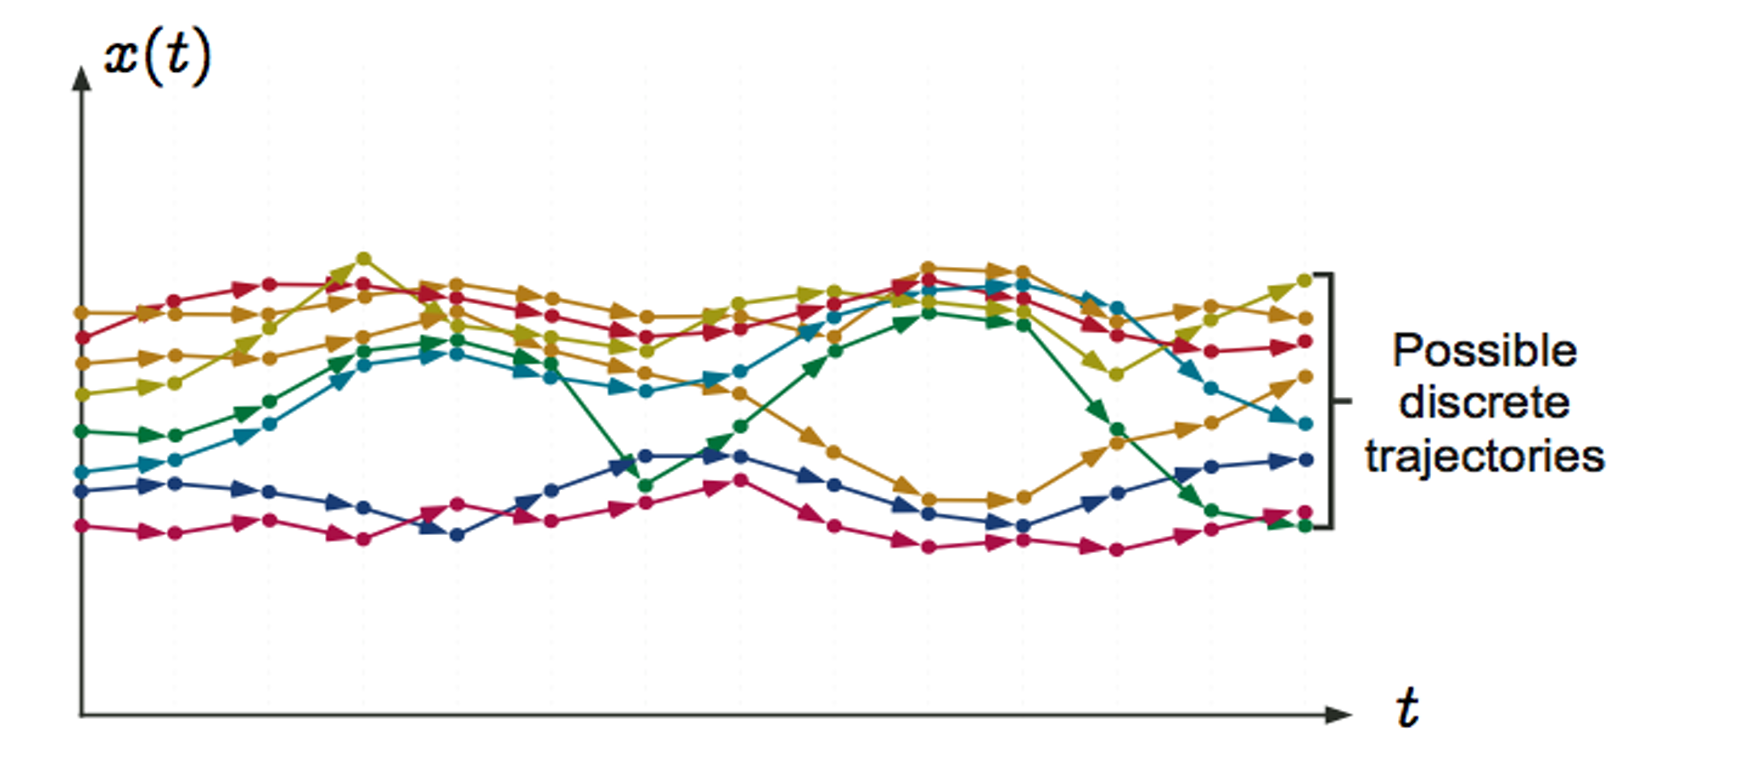
\includegraphics[scale=0.5]{img/collezionetacce.png}
\end{figure}

\section{Semantica come punto fisso}
\begin{tcolorbox}[title={Semantica a punto fisso}]
  Dato un dominio $D$ di stati e una funzione $F$:
  \begin{itemize}
  \item $D$ è un ordine parziale, cioè $\langle D, \leq \rangle$ è un \textit{po-set}, dove $D$ soddisfa le seguenti proprietà:
  \begin{itemize}
      \item Riflessività: $\forall x \in D: x \leq x$.
      \item Antisimmetria: $\forall x, y \in D: (x \leq y \land y \leq x) \Rightarrow x = y$.
      \item Transitività: $\forall x, y, z \in D: (x \leq y \land y \leq z) \Rightarrow x \leq z$.
  \end{itemize}
  \item $F: D \rightarrow D$ è una funzione totale e monotona, il che significa che per ogni $x$ e $y$ in $D$ se $x \leq y$, allora $F(x) \leq F(y)$. Inoltre, la funzione $F$ è iterabile, cioè può essere composta con se stessa più volte, ottenendo $F^n(x) = F(F(F(\ldots F(x)))$.
  \end{itemize}
  \end{tcolorbox}
  
  Un sistema di transizione è una coppia $\langle \Sigma, \tau \rangle$, dove $\Sigma$ è un insieme non vuoto di stati e $\tau$ è una relazione di transizione che collega gli stati. In altre parole, un sistema di transizione rappresenta un insieme di stati e le relazioni tra di essi, ed è utilizzato per descrivere il comportamento di sistemi o programmi.
\subsection{Punto fisso inferiore}
\begin{itemize}
  \item Il punto rosso \textcolor{red}{$\odot$} rappresenta un stato 
  bloccato.
  \item Il punto blu \textcolor{blue}{$\bullet$} rappresenta uno stato
  non bloccato.
\end{itemize}
Quindi, possiamo rappresentare l'evoluzione del sistema attraverso iterazioni. Iniziamo con un insieme vuoto di stati $X^0$:
Nella prima iterazione, otteniamo l'insieme $X^1$ contenente uno stato bloccato:

\[
  X^0 = \varnothing
\]
Nella prima iterazione, otteniamo l'insieme $X^1$ contenente uno stato bloccato:
\[
  X^1 = \{\textcolor{red}{\odot} \} 
\]
Nella seconda iterazione, aggiungiamo uno stato non bloccato con una transizione $\tau$ dall'insieme $X^1$ all'insieme $X^2$:
\[
  X^2 = \{\textcolor{red}{\odot}, \textcolor{blue}{\bullet}\xrightarrow[]{\tau} \textcolor{red}{\odot} \} 
  \qquad \text{dove } \{\textcolor{red}{\odot}\} \cup \textcolor{blue}{\bullet}\xrightarrow[]{\tau}\{ \textcolor{red}{\odot}\}
\]
In questa iterazione, uno stato non bloccato può avanzare diventando uno stato bloccato. La notazione $\textcolor{blue}{\bullet}\xrightarrow[]{\tau}$ indica una transizione che può verificarsi.
Nella terza iterazione, continuiamo ad aggiungere stati e transizioni:
Qui vediamo che gli stati non bloccati possono ancora avanzare tramite transizioni $\tau$, ma alla fine possono diventare stati bloccati.

Tutti gli stati contenuti in $X^3$ rappresentano gli stati terminati del sistema, ossia quegli stati in cui il sistema non può avanzare ulteriormente.

Qui vediamo che gli stati non bloccati possono ancora avanzare tramite
transizioni $\tau$, ma alla fine possono diventare stati bloccati.

Tutti gli stati contenuti in $X^3$ rappresentano gli stati terminati
del sistema, ossia quelli in cui il sistema non può avanzare ulteriormente.

La notazione finale, $\textit{lfp}^{\subseteq}_{\varnothing}F^+$,
rappresenta il calcolo del punto fisso inferiore di una funzione o di
un operatore $F$ in questo contesto. In questo calcolo, stiamo cercando
il più piccolo insieme di stati che rimane invariato quando applichiamo
l'operatore $F$ iterativamente a partire da un insieme vuoto. Questo è
fondamentale per identificare gli stati stabili o terminali in un sistema
o un processo.
\subsection{Punto fisso superiore}
\begin{itemize}
  \item Il punto rosso \textcolor{red}{$\odot$} rappresenta uno stato
  bloccato.
  \item Il punto blu \textcolor{blue}{$\bullet$} rappresenta uno stato
  non bloccato.
  \item Il punto arancione \textcolor{orange}{$\bullet$} rappresenta uno
  stato non bloccato che può avanzare e diventare uno stato bloccato.
\end{itemize}
Ora, possiamo rappresentare l'evoluzione del sistema attraverso
iterazioni. Iniziamo con un insieme iniziale $X^0$ che contiene
uno stato non bloccato che può avanzare e diventare uno stato bloccato, con un 
numero di passi non definito:
\[
  X^0 = \{ \textcolor{orange}{\bullet}, \textcolor{orange}{\bullet} \xrightarrow[]{?}\textcolor{orange}{\bullet},
  \textcolor{orange}{\bullet} \xrightarrow[]{?}\textcolor{orange}{\bullet}\xrightarrow[]{?}\textcolor{orange}{\bullet},
  \dots,
  \textcolor{orange}{\bullet} \xrightarrow[]{?}\textcolor{orange}{\bullet}
  \dots
  \textcolor{orange}{\bullet} \xrightarrow[]{?}\textcolor{orange}{\bullet}
  ,\dots\}
\]
Nella prima iterazione, otteniamo l'insieme $X^1$, che include uno stato
bloccato e uno stato non bloccato che può avanzare tramite una transizione
$\tau$:

\[
  X^1 = \{ \textcolor{red}{\odot}, \textcolor{blue}{\bullet} \xrightarrow[]{\tau}\textcolor{orange}{\bullet},
  \textcolor{blue}{\bullet} \xrightarrow[]{\tau}\textcolor{orange}{\bullet}\xrightarrow[]{?}\textcolor{orange}{\bullet},
  \dots,
  \textcolor{blue}{\bullet} \xrightarrow[]{\tau}\textcolor{orange}{\bullet}
  \dots
  \textcolor{orange}{\bullet} \xrightarrow[]{?}\textcolor{orange}{\bullet}
  ,\dots\}
\]
Nella seconda iterazione, otteniamo l'insieme $X^2$, che include uno
stato bloccato, uno stato non bloccato che può avanzare tramite una
transizione $\tau$, e uno stato non bloccato che può continuare a
evolversi:
\[
  X^2 = \{ \textcolor{red}{\odot}, \textcolor{blue}{\bullet} \xrightarrow[]{\tau}\textcolor{red}{\odot},
  \textcolor{blue}{\bullet} \xrightarrow[]{\tau}\textcolor{blue}{\bullet} \xrightarrow[]{\tau}\textcolor{orange}{\bullet},
  \dots,
  \textcolor{blue}{\bullet} \xrightarrow[]{\tau}\textcolor{blue}{\bullet} \xrightarrow[]{\tau}
  \textcolor{orange}{\bullet}
  \dots
  \textcolor{orange}{\bullet} \xrightarrow[]{?}\textcolor{orange}{\bullet}
  ,\dots\}
\]
Qui vediamo che gli stati non bloccati possono avanzare tramite transizioni $\tau$, ma alla fine possono diventare stati bloccati.

L'insieme $\{\textcolor{red}{\odot}\} \cup \textcolor{blue}{\bullet}\xrightarrow[]
{\tau} \Sigma^{+}$ rappresenta il punto fisso superiore
(\textit{gfp}) in questo contesto. Il \textit{gfp} rappresenta il
più grande insieme di stati che rimane invariato quando applichiamo
l'operatore $\Sigma^{+}$ iterativamente a partire da un insieme
vuoto. In altre parole, è l'insieme più grande in cui gli stati
non bloccati possono continuare a evolversi. Il \textit{gfp} è
fondamentale per identificare gli stati stabili o terminali in un
sistema o un processo.
\[
  \textit{gfp}^{\subseteq}_{\Sigma^\omega}F^\omega
\]

\subsection{Semantica dei comandi come punto fisso}
La semantica dei comandi mappa un insieme di input in un 
insieme di stati.
\[
  \llbracket \mathbb{C} \rrbracket_\wp : \wp{P}(\mathbb{M}) \rightarrow \wp(\mathbb{M})
\]
\[
  \llbracket \texttt{skip} \rrbracket_\wp(M) = M
\]
\[
  \llbracket {C_0;C_1} \rrbracket_\wp(M) = \llbracket {C_1} \rrbracket_\wp(\llbracket {C_0} \rrbracket_\wp(M))
\]
\[
  \llbracket {\texttt{x:= E}} \rrbracket_\wp(M) = \{m[x \mapsto \llbracket {E} \rrbracket_M(m)] \mid m \in M\}
\]
\[
  \llbracket \texttt{input(x)} \rrbracket_\wp(M) = \{m[x \mapsto n] \mid m \in M, n \in \mathbb{V}\}
\]
\[
  \llbracket {\texttt{if B then C else C'}} \rrbracket_\wp(M) = \llbracket C_0 \rrbracket_\wp 
  (\mathcal{F}_B (M)) \cup \llbracket C_1 \rrbracket_\wp (\mathcal{F}_{\neg B} (M))
\]
\[
  \llbracket {\texttt{while B do C}} \rrbracket_\wp(M) = \mathcal{F}_{\neg B}
  \left ( \bigcup_{i \geq 0}(\llbracket C \rrbracket_\wp \circ 
  \mathcal{F}_B)^i (M)\right )
\]
Dove:
\[
  \mathcal{F}_B(M)= \{m \in M | 
  \llbracket B \rrbracket (m) = \texttt{true}\}
\]
\subsubsection{Semantica del ciclo}
Dobbiamo partizionare l'esecuzione basandola sul numero di iterazioni
che il ciclo esegue prima di uscire.
L'insieme degli output è l'infinita unione della famiglia di insiemi $M_i$
che denotano gli stati prodotti dal programma in esecuzione.
\[
  M_i = \mathcal{F}_{\neg B}\left ( (\llbracket C \rrbracket_\wp \circ \mathcal{F}_B)^i (M)\right )
\]
Dove:
\[
\bigcup_{i \geq 0}M_i = \bigcup_{i\geq 0} \mathcal{F}_{\neg B}\left ( (\llbracket C \rrbracket_\wp \circ \mathcal{F}_B)^i (M)\right )
= \mathcal{F}_{\neg B}\left ( \bigcup_{i \geq 0}(\llbracket C \rrbracket_\wp \circ \mathcal{F}_B)^i (M)\right )
\]
Notiamo che:
\[
  \mathcal{F}_{\neg B}(\textit{lfp}_M F) \textit{ dove }F : M' \mapsto M \cup \llbracket C \rrbracket_\wp  \circ (\mathcal{F}_B(M'))
\]

\section{Il Control Flow Graph}
Il \textit{Control Flow Graph} (CFG) è un grafo diretto che rappresenta il
flusso di controllo di un programma. Il grafo è generato dalla 
sintassi del programma. Lo scopo principale di tale grafo è quello di 
permettere di capire facilmente la struttura del codice rilevando 
codice morto, cicli infiniti, e altre caratteristiche del programma.
È quindi utile per l'analisi statica del codice.

Il \texttt{CFG} è un grafo diretto $G = (N,E)$ dove:
\begin{itemize}
  \item un nodo $n \in N$ rappresenta un blocco di codice, ovvero è una sequenza massimale
  di istruzioni con un singolo punto di ingresso, 
  un singolo punto di uscita e senza diramazioni interne.
  Per semplicità, assumiamo un unico nodo d'ingresso $n_0$ e un unico nodo di uscita $n_f$.
  \item Un arco $e=(n_i,n_j) \in E$ rappresenta un possibile flusso di controllo tra due blocchi di codice.
\end{itemize}
\begin{figure}[H]
  \begin{subfigure}{0.5\textwidth}
    \centering
    \begin{tikzpicture}[->,>=stealth,shorten >=1pt,auto,node distance=3cm,
      thick,block/.style={rectangle, draw, text width=2cm, text centered, minimum height=1cm}]
    
    \node[block] (1) {if(x == y)};
    \node[block] (2) [below left of=1] {then \{...\}};
    \node[block] (3) [below right of=1] {else \{...\}};
    \node[block] (4) [below right of=2] {...};
    
    \path[every node/.style={font=\sffamily\small}]
    (1) edge node {} (2)
    edge node {} (3)
    (2) edge node {} (4)
    (3) edge node {} (4);
    \end{tikzpicture}
    \caption{Esempio di CFG}
  \end{subfigure}
  \begin{subfigure}{0.5\textwidth}
    \centering
    \begin{verbatim}
      if(x == y)
          then
              ...
          else
              ...
      ...
      \end{verbatim}
  \end{subfigure}
  \caption{La figura generale}
\end{figure}
\subsection{Blocchi di base}
\begin{tcolorbox}[title=Blocco di base]
  Un blocco di base è la massima sequenza consecutiva di istruzioni senza 
  diramazioni interne, con un singolo punto di ingresso, un singolo punto di uscita
  e senza salti all'interno del blocco.
\end{tcolorbox}
Si tratta dell'unità di base per la costruzione del \verb|CFG| e per l'analisi del flusso.

Le ottimizzazioni che è possibile attuare includono
l'eliminazione della ridondanza e l'allocazione dei registri.
\subsection{Identificare i blocchi di base}
Questo è un processo di analisi del flusso di controllo per identificare i blocchi di base. Di seguito è riportata una spiegazione dettagliata basata sull'input fornito:

\textbf{Identificazione dei leader:}
\begin{itemize}[label=--,topsep=0pt,itemsep=0pt]
  \item Il primo statement nella sequenza (\textit{punto di ingresso}) è un leader.
  \item Ogni statement ``s" che è la destinazione di un salto
  (\textit{condizionale o incondizionale}) è un leader (\textit{cioè esiste un ``goto s"}).
  \item Ogni statement immediatamente successivo a un salto
  (\textit{condizionale o incondizionale}) o a un return è un leader.
\end{itemize}

\textbf{Creazione dei blocchi di base:}
\begin{itemize}
  \item Per ogni leader identificato, il suo blocco di base include
  il leader stesso e tutte le istruzioni fino al prossimo leader
  (\textit{senza includerlo}) o fino alla fine del programma.
\end{itemize}

Questo processo consente di identificare i blocchi di base e di definire
il flusso di controllo all'interno del programma.

\subsection{Esempio}
\begin{figure}[H]
  \centering
  \begin{tikzpicture}[node distance=0.3cm and 6cm]
    \node (1) {1. \texttt{i := m - 1}};
    \node [below=of 1] (2) {2. \texttt{j := n}};
    \node [below=of 2] (3) {3. \texttt{t1 := 4 * n}};
    \node [below=of 3] (4) {4. \texttt{v := a[t1]}};
    \node [below=of 4] (5) {5. \texttt{i := m + 1}};
    \node [below=of 5] (6) {6. \texttt{t2 := 4 * i}};
    \node [below=of 6] (7) {7. \texttt{t3 := a[t2]}};
    \node [below=of 7] (8) {8. \texttt{if t3 < v goto (5)}};
    \node [below=of 8] (9) {9. \texttt{j:= j - 1}};
    \node [below=of 9] (10) {10. \texttt{t4 := 4 * j}};
    \node [below=of 10] (11) {11. \texttt{t5 := a[t4]}};
    \node [below=of 11] (12) {12. \texttt{if t5 > v goto (9)}};
    \node [below=of 12] (13) {13. \texttt{if i >= j goto (23)}};
    \node [below=of 13] (14) {14. \texttt{t6 := 4 * i}};
    \node [below=of 14] (15) {15. \texttt{x := a[t6]}};
  
    \node [right=of 1]  (16) {16. \texttt{t7 := 4 * i}};
    \node [below=of 16] (17) {17. \texttt{t8 := 4 * j}};
    \node [below=of 17] (18) {18. \texttt{t9 := a[t8]}};
    \node [below=of 18] (19) {19. \texttt{a[t7] := t9}};
    \node [below=of 19] (20) {20. \texttt{t10 := 4 * j}};
    \node [below=of 20] (21) {21. \texttt{a[t10] := x}};
    \node [below=of 21] (22) {22. \texttt{goto (5)}};
    \node [below=of 22] (23) {23. \texttt{t11 := 4 * i}};
    \node [below=of 23] (24) {24. \texttt{x := a[t11]}};
    \node [below=of 24] (25) {25. \texttt{t12 := 4 * i}};
    \node [below=of 25] (26) {26. \texttt{t13 := 4 * n}};
    \node [below=of 26] (27) {27. \texttt{t14 := a[t13]}};
    \node [below=of 27] (28) {28. \texttt{a[t12] := t14}};
    \node [below=of 28] (29) {29. \texttt{t15 := 4 * n}};
    \node [below=of 29] (30) {30. \texttt{a[t15] := x}};
    \node [fit=(current bounding box), draw, inner sep=0.5cm] (box) {};
  \end{tikzpicture}
\end{figure}

\begin{figure}[H]
  \centering
  \begin{tikzpicture}[node distance=0.1cm and 6cm]
    \node (1) {1. \texttt{i := m - 1}};
    \node [below=of 1, draw=red, thick, minimum width=1.5cm] (2) {2. \texttt{j := n}};
    \node [below=of 2] (3) {3. \texttt{t1 := 4 * n}};
    \node [below=of 3] (4) {4. \texttt{v := a[t1]}};
    \node [below=of 4, draw=red, thick, minimum width=1.5cm] (5) {5. \texttt{i := m + 1}};
    \node [below=of 5] (6) {6. \texttt{t2 := 4 * i}};
    \node [below=of 6] (7) {7. \texttt{t3 := a[t2]}};
    \node [below=of 7] (8) {8. \texttt{if t3 < v goto (5)}};
    \node [below=of 8, draw=red, thick, minimum width=1.5cm] (9) {9. \texttt{j:= j - 1}};
    \node [below=of 9] (10) {10. \texttt{t4 := 4 * j}};
    \node [below=of 10] (11) {11. \texttt{t5 := a[t4]}};
    \node [below=of 11] (12) {12. \texttt{if t5 > v goto (9)}};
    \node [below=of 12, draw=red, thick, minimum width=1.5cm] (13) {13. \texttt{if i >= j goto (23)}};
    \node [below=of 13, draw=red, thick, minimum width=1.5cm] (14) {14. \texttt{t6 := 4 * i}};
    \node [below=of 14] (15) {15. \texttt{x := a[t6]}};
  
    \node [right=of 1]  (16) {16. \texttt{t7 := 4 * i}};
    \node [below=of 16] (17) {17. \texttt{t8 := 4 * j}};
    \node [below=of 17] (18) {18. \texttt{t9 := a[t8]}};
    \node [below=of 18] (19) {19. \texttt{a[t7] := t9}};
    \node [below=of 19] (20) {20. \texttt{t10 := 4 * j}};
    \node [below=of 20] (21) {21. \texttt{a[t10] := x}};
    \node [below=of 21] (22) {22. \texttt{goto (5)}};
    \node [below=of 22, draw=red, thick, minimum width=1.5cm] (23) {23. \texttt{t11 := 4 * i}};
    \node [below=of 23] (24) {24. \texttt{x := a[t11]}};
    \node [below=of 24] (25) {25. \texttt{t12 := 4 * i}};
    \node [below=of 25] (26) {26. \texttt{t13 := 4 * n}};
    \node [below=of 26] (27) {27. \texttt{t14 := a[t13]}};
    \node [below=of 27] (28) {28. \texttt{a[t12] := t14}};
    \node [below=of 28] (29) {29. \texttt{t15 := 4 * n}};
    \node [below=of 29] (30) {30. \texttt{a[t15] := x}};
  
    \node [fit=(current bounding box), draw, inner sep=0.5cm] (box) {};
  \end{tikzpicture}
\end{figure}

La partizione del codice intermedio in blocchi di base coinvolge diversi passaggi
importanti per rappresentare il flusso di controllo in un programma. I passaggi
chiave sono i seguenti:

\begin{itemize}
  \item Aggiunta di archi corrispondenti ai flussi di controllo tra i blocchi.
  \item Trattamento dei costrutti come:
  \begin{itemize}
    \item \textbf{Goto incondizionale}: Questo genera un collegamento diretto a
    un blocco specifico.
    \item \textbf{Branch condizionale}: Può generare più archi uscenti da un blocco,
    a seconda delle possibili condizioni.
    \item \textbf{Flusso sequenziale}: Se non ci sono ramificazioni alla fine di un blocco,
    il controllo passa semplicemente al blocco successivo.
  \end{itemize}
  \item Aggiunta di nodi finti e archi, se necessario, per rappresentare i nodi di ingresso
  e di uscita nel caso in cui non siano unici.
  \item L'obiettivo è di semplificare al massimo gli algoritmi di analisi e trasformazione,
  assicurando che non ci siano archi che entrano nel nodo di ingresso $n_0$ o che escono dal
  nodo di uscita $n_f$.
\end{itemize}

Questi passaggi sono cruciali per modellare accuratamente il flusso di controllo all'interno
di un programma e facilitare ulteriori analisi e ottimizzazioni.
\begin{figure}[H]
  \centering
  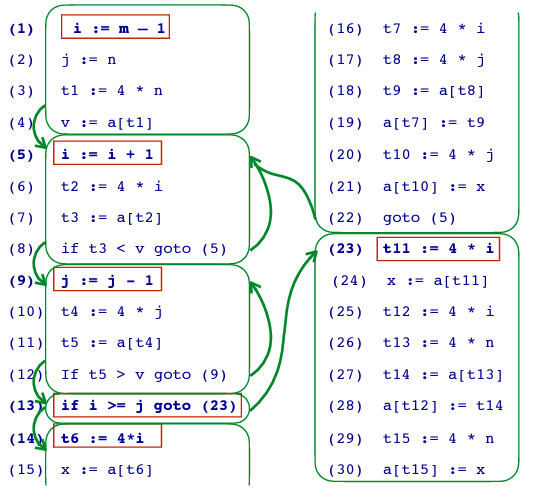
\includegraphics[width=0.6\textwidth]{img/cfg.png}
\end{figure}
Dato un \verb|CFG| = $\langle N, E\rangle$, 
è definito come un insieme di nodi e archi,
dove ogni arco rappresenta il flusso di controllo
tra due nodi. Nel contesto di un $\texttt{CFG} = <N, E>:$
\begin{itemize}
  \item Se esiste un arco $n_i$ $\rightarrow$ $n_j$ $\in$ $E$:
  \begin{itemize}
    \item $n_i$ è un predecessore di $n_j$
    \item $n_j$ è un successore di $n_i$
  \end{itemize}
  \item Per qualsiasi nodo $n \in N$:
  \begin{itemize}
    \item \texttt{Pred(n)}: l'insieme dei predecessori di $n$
    \item \texttt{Succ(n)}: l'insieme dei successori di $n$
    \item Un nodo di diramazione (\texttt{branch node}) è un nodo che ha più di un successore
    \item Un nodo di unione, (\texttt{join node}) è un nodo che ha più di un predecessore
  \end{itemize}
\end{itemize}
\section{Il linguaggio \texttt{imp-CFG}}
Spostando la caratteristica di controllo sulla struttura del grafo,
il linguaggio non è più \verb|IMP|, ma una versione leggermente modificata:
\begin{itemize}
    \item I vertici corrispondono ai punti del programma
    \item Gli archi sono passi del calcolo etichettati con l'azione del programma corrispondente
    \item Le etichette delle istruzioni diventano etichette dei nodi
\end{itemize}
\[
  \begin{array}{lcl}
    \textbf{test:} & \texttt{NonZero(e)} \text{ or } \texttt{Zero(e)} \\
    \textbf{assignment:} & x \leftarrow e \\
    \textbf{empty statement:} & ; \\
    \textbf{input:} & \texttt{input(x)} \\
    \end{array}
\]
\subsubsection{Esempio}
\begin{figure}[H]
  \begin{subfigure}{0.5\textwidth}
    \begin{verbatim}
      input(x);
      y := 2;
      while(x > 0) {
        y := y + 2;
        x := x - 1;
      }
    \end{verbatim}
  \end{subfigure}
  \begin{subfigure}{0.5\textwidth}
    \begin{tikzpicture}[node distance={22mm}, main/.style = {draw, circle}] 
      \node[main] (0) {$0$}; 
      \node[main] (1) [below =of 0] {$1$};
      \node[main] (2) [below =of 1] {$2$};
      \node[main] (5) [right =of 2] {$5$};
      \node[main] (4) [below right =of 5] {$4$};
      \node[main] (3) [below left =of 4] {$3$};
      %%cerchio doppio per il 6
      \node[main] (6) [below =of 2] {$6$};
      \draw[->] (0) to node[left] {\small\texttt{input(x)}} (1);
      \draw[->] (1) to node[left] {$y \leftarrow 2$} (2);
      \draw[->] (2) to node[above right] {\small \texttt{NonZero(x > 0)}} (3);
      \draw[->] (2) to node[left] {\small \texttt{Zero(x > 0)}} (6);
      \draw[->] (3) to node[below right] {$y \leftarrow y + 2$} (4);
      \draw[->] (4) to node[above right] {$x \leftarrow x - 1$} (5);
      \draw[->] (5) to node[above] {;} (2);
      \end{tikzpicture}
  \end{subfigure}
\end{figure} 

Una dichiarazione condizionale o un ciclo all'interno di un grafo di flusso di controllo
presenta due archi corrispondenti: l'arco etichettato con \texttt{NonZero} viene percorso se
la condizione ``e" è verificata (cioè se ``e" viene valutata come un valore diverso da $0$).
L'arco etichettato con \texttt{Zero}, invece, viene percorso se la condizione non è soddisfatta.

Un arco è definito come $k=(u,\texttt{lab},v)$, dove $u$ rappresenta il vertice di partenza,
$v$ rappresenta il vertice di destinazione e \texttt{lab} rappresenta l'etichetta dell'arco.
Questo arco rappresenta l'effetto della dichiarazione, ovvero la trasformazione dello stato prima
dell'esecuzione dell'azione di etichettatura in uno stato successivo: \textbf{effetto dell'arco}.
\subsection{Semantica del linguaggio \texttt{imp-CFG}}
La semantica del linguaggio descrive la trasformazione dello stato prima e dopo l'esecuzione di
un'azione del linguaggio, che viene riflessa nell'effetto complessivo della dichiarazione all'interno
del programma.
\[
\begin{array}{lcl}
  \llbracket ; \rrbracket(m) & = & m \\
  \llbracket \texttt{NonZero(e)} \rrbracket(m) & = & m \qquad \textit{if } \llbracket e \rrbracket(m) = \texttt{true} \\
  \llbracket \texttt{Zero(e)} \rrbracket(m) & = & m \qquad \textit{if } \llbracket e \rrbracket(m) = \texttt{false} \\
  \llbracket x \leftarrow e \rrbracket(m) & = & m[x \mapsto \llbracket e \rrbracket(m)] \\
  \llbracket \texttt{input(x)} \rrbracket(m) & = & m[x \mapsto m(x)] \\
\end{array}
\] 
\subsection{Computazione del linguaggio \texttt{imp-CFG}}
Una computazione è un percorso nel grafo di flusso di controllo, ovvero una sequenza di archi
che iniziano dal nodo iniziale $u$ e terminano in un nodo finale $v$. Il percorso è quindi 
una sequenza di archi:
\[
  \pi = k_1, k_2, \dots, k_n = (u_i, \texttt{lab}_i, u_{i+1}), i = 1, \dots, n - 1, u = u_1, v = v_n
\]
La trasformazione di stato corrispondente alle computazioni ottenuta dalla
composizione degli effetti degli archi della computazione:
\[
  \llbracket \pi \rrbracket = \llbracket k_n \rrbracket \circ \dots \circ \llbracket k_1 \rrbracket
\]

\chapter{Significato di approssimare}
\section{L'idea di approssimazione}
Immagina di avere due insiemi di oggetti: uno di questi, chiamiamolo $\llbracket P \rrbracket$,
ha una caratteristica speciale che chiameremo $Q$. Ora, il punto cruciale è che non possiamo dire
con certezza se un determinato oggetto appartiene a $Q$ o meno. È come se avessimo un mucchio di
oggetti e non riuscissimo a dire se uno specifico oggetto appartiene a un gruppo particolare o meno.

Quello che dobbiamo fare è trovare un modo per approssimare l'insieme $\llbracket P \rrbracket$
in modo da poter prendere decisioni più facili su $Q$. In altre parole, dobbiamo trovare un altro
insieme, $\llbracket P \rrbracket^\sharp$, che contiene la maggior parte degli oggetti di $\llbracket P \rrbracket$,
ma che sia più facile da analizzare. Questo insieme deve avere due caratteristiche importanti: tutti gli
oggetti di $\llbracket P \rrbracket$ devono essere anche in $\llbracket P \rrbracket^\sharp$, e l'insieme
$\llbracket P \rrbracket^\sharp$ deve essere tale che possiamo dire con certezza se un oggetto appartiene a $Q$ o meno.

Quando abbiamo questo insieme $\llbracket P \rrbracket^\sharp$, possiamo utilizzarlo per fare deduzioni
su $Q$. Se tutti gli oggetti in $\llbracket P \rrbracket^\sharp$ appartengono a $Q$, allora possiamo dire
con sicurezza che tutti gli oggetti in $\llbracket P \rrbracket$ devono appartenere a $Q$. Ma se non
tutti gli oggetti in $\llbracket P \rrbracket^\sharp$ appartengono a $Q$, non possiamo essere certi se gli
oggetti in $\llbracket P \rrbracket$ appartengono o meno a $Q$.

In sostanza, il nostro obiettivo è rendere più facile prendere decisioni su questi oggetti, anche se non
possiamo dire con certezza assoluta se un oggetto specifico appartiene a $Q$. Questo approccio ci consente
di ragionare in modo più chiaro su questi insiemi e di trarre conclusioni ragionevoli su di essi.

La correttezza ci consente di sfruttare la decidibilità dell'approssimazione:
\[
  \llbracket P \rrbracket \subseteq Q \implies \llbracket P \rrbracket^\sharp \subseteq Q  
\]
Altrimenti, non possiamo saperlo con certezza!
\subsection{Astrazione della semantica}
Vediamo come costruire l'insieme $\llbracket P \rrbracket^\sharp$ a partire da $\llbracket P \rrbracket$.
Specificheremo la semantica come una coppia: una funzione $f$ (\textit{con punto fisso}) e un
dominio di calcolo $D$ (\textit{ordinato}).

\begin{itemize}
  \item Astrazione del dominio di calcolo e delle relazioni tra oggetti concreti e astratti, ovvero 
  l'osservazione astratta dei dati e come questi si relazionano tra loro.
  \item Astrazione del calcolo, con particolare attenzione all'astrazione del punto fisso, come la 
  semantica manipola questi risultati astratti.
\end{itemize}
L'astrazione è il processo di sostituire qualcosa di concreto con una descrizione che considera alcune proprietà
(\textit{generalmente non tutte}), definita come modello astratto.
Può descrivere alcune proprietà in modo preciso, ma non tutte.

Un'astrazione $\wp(\Sigma)$ di oggetti in $\Sigma$ è $A \subseteq \wp(\Sigma)$ tale che:
\begin{itemize}
    \item Gli elementi presenti nell'insieme $A$ sono quelli descritti precisamente
    dall'astrazione, senza perdita di precisione.
    \item Gli elementi non presenti nell'insieme $A$ devono essere rappresentati da
    altri elementi dell'insieme, con una perdita di precisione.
\end{itemize}
\subsection{Oggetti}
Nell'analisi/verifica dei programmi dobbiamo considerare oggetti che rappresentano parti dello stato di calcolo:
\begin{itemize}
    \item Valori: Booleani, Interi,... $\mathcal{V}$
    \item Nomi di variabili $\mathbb{X}$
    \item Ambienti $\mathbb{X} \rightarrow \mathcal{V}$
    \item Stacks
    \item $\ldots$
\end{itemize}
\subsubsection{Proprietà}
Le proprietà sono insiemi di oggetti (che hanno quella proprietà). Esempi:
\begin{itemize}
    \item Numeri naturali dispari: $\{1, 3, 4, \dots, 2n + 1, \dots\}$
    \item Numeri interi pari: $\{2z \mid z \in \mathbb{Z}\}$
    \item Valori delle variabili intere: $\{x \mid x \in \mathbb{X} \land \texttt{minint} < x < \texttt{maxint}\}$
    \item Proprietà di invarianza: di un programma con stati: $\Gamma$
    \[
      I \in \wp(\Sigma)
    \]
    \item $\ldots$
\end{itemize}
\subsection{Proprietà}
L'insieme delle proprietà di $\wp(\Sigma)$ degli oggetti in $\Sigma$ è un reticolo distributivo completo, 
\[
  \langle \wp(\Sigma), \subseteq, \varnothing, \sigma, \Sigma, \cup, \cap, \neg  \rangle 
\]
Nell'analisi di un sistema complesso, è essenziale considerare l'astrazione come un processo chiave
per semplificare la comprensione. Quando si tratta di approssimare una proprietà concreta con
un'astrazione, si aprono due possibili approcci.
L'approccio di \textbf{approssimazione dal basso} implica che l'astrazione rappresenti un sottoinsieme
della proprietà concreta,
mentre l'approccio di \textbf{approssimazione dall'alto} ($P$) implica che l'astrazione rappresenti un
sovrainsieme della proprietà concreta. Questi approcci possono essere visti come duali,
sebbene l'analisi si concentri principalmente sull'approccio di approssimazione dall'alto,
poiché trovare approssimazioni utili dal basso può essere più impegnativo e complesso.

\begin{figure}[H]
  \centering
  \begin{tikzpicture}[scale=0.8]
    % Nodes
    \node (top) at (0,2) {$\Sigma$};
    \node (a) at (-2,0) {$\alpha$};
    \node (b) at (2,0) {$\beta$};
    \node (bottom) at (0,-2) {$\varnothing$};
    % Lines
    \draw (top) -- (a) -- (bottom);
    \draw (top) -- (b) -- (bottom);
    \draw (a) -- (b);
  \end{tikzpicture}
\end{figure}
\subsubsection{Least upper bound}
Il least upper bound (\verb|LUB|) di un insieme di elementi è il più piccolo
elemento del reticolo che è maggiore o uguale a ciascun elemento dell'insieme ($X \lor Y$).
Ovvero in $\wp(D)$ tale che $A \supseteq X$ e $A \supseteq Y$.
\begin{figure}[H]
  \centering
  \begin{tikzpicture}[scale=0.8]
    % Nodes
    \node (from-y-to-x) at (-2, 5) {};
    \node (from-x-to-y) at (2, 5) {};
    \node (inters) at (0,2.5) {};
    \node (x-side) at (-5.5,5) {};
    \node (y-side) at (5.5,5) {};
    \node (x) at (-2,0) {$x$};
    \node (y) at (2,0) {$y$};

    %colorare l'area 
    \fill[blue!20] (0,2.5) -- (from-x-to-y.center) -- (from-y-to-x.center) -- cycle;
    

    % Lines
    \draw (x) -- (from-x-to-y);
    \draw (y) -- (from-y-to-x);
    \draw (x) -- (x-side);
    \draw (y) -- (y-side);

    \draw[fill=red] (0,2.5) circle (5pt);
    
  \end{tikzpicture}
\end{figure}
\subsubsection{Greatest lower bound}
Il greatest lower bound (\verb|GLB|) di un insieme di elementi è il più grande
elemento del reticolo che è minore o uguale a ciascun elemento dell'insieme ($X \land Y$).
Ovvero in $\wp(D)$ tale che $A \subseteq X$ e $A \subseteq Y$.
\begin{figure}[H]
  \centering
  \begin{tikzpicture}[scale=0.8]
    % Nodes
    \node (from-y-to-x) at (-2, -5) {};
    \node (from-x-to-y) at (2, -5) {};
    \node (inters) at (0,-2.5) {};
    \node (x-side) at (-5.5,-5) {};
    \node (y-side) at (5.5,-5) {};
    \node (x) at (-2,0) {$x$};
    \node (y) at (2,0) {$y$};

    %colorare l'area 
    \fill[blue!20] (0,-2.5) -- (from-x-to-y.center) -- (from-y-to-x.center) -- cycle;
    

    % Lines
    \draw (x) -- (from-x-to-y);
    \draw (y) -- (from-y-to-x);
    \draw (x) -- (x-side);
    \draw (y) -- (y-side);

    \draw[fill=red] (0,-2.5) circle (5pt);
    
  \end{tikzpicture}
\end{figure}
\section{Approssimazione dei dati}
Sia $P^\sharp$ una proprietà di $D$ se e solo se $P^\sharp$ e $\wp(D)$. Vogliamo quindi capire la relazione tra gli 
elementi di $D$ e $\wp(D)$ e poi, preso $D^\sharp \subseteq \wp(D)$ la relazione tra gli elementi di $D$ e gli elementi 
di $D^\sharp$.
Per approssimare $D$ scegliamo un sottoinsieme $D^\sharp$ che fissa le proprietà che vogliamo osservare (\textit{con precisione}).
In generale $d \in D \implies d^\sharp \in D \subseteq \wp(D)$.

Potremmo quindi avere:
\begin{itemize}
  \item $d \subseteq d^\sharp$ ovvero \textbf{over approximation}.
  \item $d \supseteq d^\sharp$ ovvero \textbf{under approximation}.
\end{itemize}
\subsection{Approssimazione dal basso}
\begin{figure}[H]
  \centering
  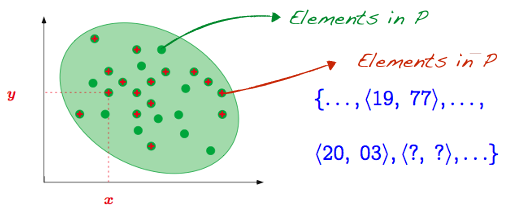
\includegraphics[scale=0.5]{img/approx.png}
\end{figure}
Per rispondere alla domanda $\langle x, y \rangle \in P$ utilizziamo un'astrazione $\bar{P}$,
tale che $P \supseteq \bar{P}$.
\begin{itemize}
  \item Se $\langle x, y \rangle \in \bar{P}$, quindi $d \subseteq d^\sharp$, allora $\langle x, y \rangle \in P$.
  \item Se $\langle x, y \rangle \notin \bar{P}$, quindi $d \supseteq d^\sharp$, allora non lo sappiamo.
\end{itemize}
In sintesi prendiamo un insieme più piccolo che comprende una sottoparte del nostro insieme di partenza e
analizziamo tale insieme più piccolo. Se troviamo una risposta positiva allora abbiamo risposto alla domanda,
altrimenti non lo sappiamo.
\subsection{Approssimazione dall'alto}
\begin{figure}[H]
  \centering
  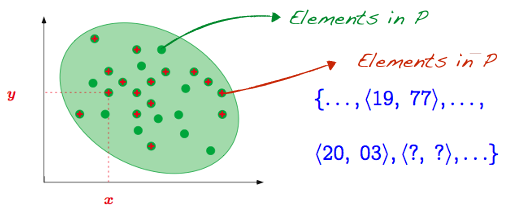
\includegraphics[scale=0.5]{img/approx.png}
\end{figure}
Per rispondere alla domanda $\langle x, y \rangle \in P$ utilizziamo un'astrazione $\bar{P}$,
tale che $P \subseteq \bar{P}$.
\begin{itemize}
  \item Se $\langle x, y \rangle \in \bar{P}$, quindi $d \supseteq d^\sharp$, allora non sappiamo rispondere.
  \item Se $\langle x, y \rangle \notin \bar{P}$, quindi $d \subseteq d^\sharp$, allora no.
\end{itemize}
In sintesi prendiamo un insieme più grande che comprende il nostro insieme di partenza e
analizziamo tale insieme più grande. Più grande non è sinonimo di più complesso, ma spesso 
ricondurci a proprietà più generali potrebbe aiutarci nell'analisi, la rappresentazione estensionale 
potrebbe quindi risultare più semplice. Tale approccio ci permette 
di rispondere alla domanda solo che la proprietà non è soddisfatta per il nuovo insieme più grande, 
ovvero $P^\sharp$.

In sostanza:
\begin{tcolorbox}[title=Proprietà concrete]
Le proprietà concrete sono un insieme di oggetti potenzialmente complessi, infiniti e non rappresentabili
da un calcolatore.
\end{tcolorbox}

\begin{tcolorbox}[title=Proprietà astratte]
  Le proprietà astratte sono un insieme più ampio di oggetti. A volte, l'ampiezza maggiore
  implica una maggiore estensibilità per la rappresentazione. Tuttavia, strutture più ampie
  ben scelte possono
  avere codifiche più semplici che possono essere sfruttate per la memorizzazione e il calcolo.
\end{tcolorbox}
\subsection{Minima astrazione}
Assumendo che le proprietà astratte $P \in \wp(\Sigma)$ devono essere approssimate 
dall'alto della proprietà astratta $\bar{P} \in A \subset \wp(\Sigma)$, tale che:
\[
  P \subseteq \bar{P}
\]
Sappiamo che la più piccola proprietà $\bar{P}$ è la più precisa delle approssimazioni che possiamo avere.
Ovviamente, la minima proprietà astratta potrebbe non non esistere per tutte le astrazioni $A$.
Se questa minima approssimazione esiste è preferibile che sia il più precisa possibile, se non esiste,
può essere utilizzata una
migliore alternativa che fornisce un'approssimazione più precisa.
\subsection{Miglior astrazione}
Una buona scelta per l'astrazione è quella che fornisce la
miglior approssimazione per ogni proprietà concreta
\[
  P \subseteq \bar{P}
\]
\[
  \forall \bar{P}' \in A . (P \subseteq \bar{P}') \implies (\bar{P} \subseteq \bar{P}')
\]
Segue che la miglior approssimazione è la \textit{greatest lower bound} di tutte le approssimazioni
delle proprietà.
\[
\bar{P} = \bigcap \{\bar{P}' \in A \mid P \subseteq \bar{P}'\} \in A
\]
Tra tutti gli elementi più piccoli di quelli in $X$, è il più grande.
\[
  x = \texttt{glb}X \subseteq P \iff \forall l \in P . (\forall y \in X. l \leq y) \implies x \geq l
\]
\subsection{Esempio: \texttt{Sign}}
\subsubsection{Semantica concreta}
Abbiamo a disposizione programmi che manipolano numeri interi: \(f: \mathbb{Z} \to \mathbb{Z}\). Una delle 
proprietà osservate è quella di \textit{sign}, ovvero che il risultato tra due numeri dipenderà dal segno
dei due numeri. Dobbiamo indicare cosa inseriremo in $D^\sharp$ ovvero \texttt{Sign}.
\begin{itemize}
  \item $+ = \{n \mid n > 0\} \in \wp(\mathbb{Z})$
  \item $- = \{n \mid n < 0\} \in \wp(\mathbb{Z})$
  \item $0 = \{0\} \in \wp(\mathbb{Z})$
\end{itemize}
Quindi:
\[
  \{+, 0, -\} \subseteq \wp(\mathbb{Z})
\] 

\subsubsection{Semantica astratta}
Il dominio astratto, noto come \texttt{Sign}, viene utilizzato per approssimare
l'insieme di interi manipolati dai programmi. La funzione $f^\sharp$ manipola quindi i segni. 
\[
  D^\sharp = \{+, -, 0, \mathbb{Z}, \varnothing\} = \texttt{Sign}
\]
In \texttt{Sign},
gli interi possono essere rappresentati come:

\begin{itemize}
  \item $x \subseteq \mathbb{Z} \rightarrow x^\sharp \in D^\sharp$ è il più piccolo 
  insieme in $D^\sharp$ che contiene $x$.
  \item \(\{-,5,4 \} \rightarrow \mathbb{Z}\)
  \item \(\{ 3 \} \rightarrow + \equiv \mathbb{Z}\)
  \item \(\{ 7 \}  \rightarrow + \equiv \mathbb{Z}^{+}\)
  \item \(\{-5 \} \rightarrow - \equiv \mathbb{Z}^{-}\)
  \item \( \{ -5, -6 \} \rightarrow - \equiv \mathbb{Z}^{-}\)
\end{itemize}
\begin{minipage}[t]{0.4\textwidth}
  \begin{figure}[H]
  \centering
  \renewcommand{\arraystretch}{2}
  \begin{tabular}{|m{2em}|m{2em}|m{2em}|m{2em}|m{2em}|m{2em}|}
      \hline
       & $\mathbb{Z}$ & $\mathbb{Z}^+$ & $\mathbb{Z}^0$ & $\mathbb{Z}^-$ & $\varnothing$ \\
      \hline
      $\mathbb{Z}$ & $\mathbb{Z}$ & $\mathbb{Z}$ & $\mathbb{Z}$ & $\mathbb{Z}$ & $\mathbb{Z}$ \\
      \hline
      $\mathbb{Z}^+$ & $\mathbb{Z}$ & $\mathbb{Z}^+$ & $\mathbb{Z}^+$ & \textcolor{red}{$\mathbb{Z}$} & $\mathbb{Z}^+$ \\
      \hline
      $\mathbb{Z}^0$ & $\mathbb{Z}$ & $\mathbb{Z}^+$ & $\mathbb{Z}^0$ & $\mathbb{Z}^-$ & $\mathbb{Z}^0$ \\
      \hline
      $\mathbb{Z}^-$ & \textcolor{red}{$\mathbb{Z}$}  & $\mathbb{Z}$ & $\mathbb{Z}^-$ & $\mathbb{Z}^-$ & $\mathbb{Z}^-$ \\
      \hline
      $\varnothing$ & $\mathbb{Z}$ & $\mathbb{Z}^+$ & $\mathbb{Z}^0$ & $\mathbb{Z}^-$ & $\varnothing$ \\
      \hline
    \end{tabular}
    \caption{Operazioni di \texttt{Sign} relative alla somma.}
  \end{figure}
\end{minipage}
\hfill
\begin{minipage}[t]{0.5\textwidth}
  \begin{figure}[H]
    \centering
    \renewcommand{\arraystretch}{2}
    \begin{tabular}{|m{2em}|m{2em}|m{2em}|m{2em}|m{2em}|m{2em}|}
        \hline
        & $\mathbb{Z}$ & $\mathbb{Z}^+$ & $\mathbb{Z}^0$ & $\mathbb{Z}^-$ & $\varnothing$ \\
        \hline
        $\mathbb{Z}$ & $\mathbb{Z}$ & $\mathbb{Z}$ & $\mathbb{Z}$ & $\mathbb{Z}$ & $\mathbb{Z}$ \\
        \hline
        $\mathbb{Z}^+$ & $\mathbb{Z}$ & $\mathbb{Z}^+$ & $\mathbb{Z}^0$ & $\mathbb{Z}^-$ & $\mathbb{Z}^+$ \\
        \hline
        $\mathbb{Z}^0$ & $\mathbb{Z}$ & $\mathbb{Z}^0$ & $\mathbb{Z}^0$ & $\mathbb{Z}^0$ & $\mathbb{Z}^0$ \\
        \hline
        $\mathbb{Z}^-$ & $\mathbb{Z}$ & $\mathbb{Z}^-$ & $\mathbb{Z}^0$ & $\mathbb{Z}^+$ & $\mathbb{Z}^-$ \\
        \hline
        $\varnothing$ & $\mathbb{Z}$ & $\mathbb{Z}^+$ & $\mathbb{Z}^0$ & $\mathbb{Z}^-$ & $\varnothing$ \\
        \hline
    \end{tabular}
    \caption{Operazioni di \texttt{Sign} relative alla moltiplicazione.}
  \end{figure}
\end{minipage}

Per quanto riguarda la somma perdiamo informazioni solamente nel caso in cui si abbia un'operazione tra 
un numero positivo e uno negativo, poiché perdiamo le informazioni relative ai valori. Per quanto riguarda la moltiplicazione, invece, non perdiamo informazioni 
guardando la proprietà \texttt{Sign}, poiché è precisa sulla moltiplicazione.
\section{Astrazione delle computazioni}
Si tratta di approssimare la semantica sul dominio delle osservazioni.
Una volta fissate queste osservazioni, osserviamo come la semantica opera su di esse.

Abbiamo già visto il significato di computazione, che ripetiamo.
\begin{tcolorbox}[title = {Computazione}]
  Una computazione è una traccia nel tempo dello stato del programma durante l'esecuzione. Quindi lo stato 
  delle memorie nei vari punti del programma.
  A partire da uno stato iniziale noi abbiamo le possibili traiettorie di esecuzione del programma, 
  talvolta infinite 
  poiché potenzialmente divergenti.
\end{tcolorbox}
In realtà le possibili traiettorie non sono continue, ma sono discrete, poiché fissiamo degli step di tempo 
che tipicamente corrispondono alle singole istruzioni del programma e ogni traccia è spezzata in questa sequenza 
di evoluzione.

\subsection{Computazione di insiemi}
Quello che avviene ricerca della \textbf{decidibilità} è quello di osservare le proprietà di interesse.
Per osservare le proprietà di interesse, necessitiamo dell'osservazione di insiemi. L'insieme infatti 
rappresenta una proprietà che descrive un invariante di tutti gli elementi in esso contenuti.

Trasformando l'insieme di tracce in un'unica computazione che avviene tra insiemi. I punti rimangono comunque 
concreti, quindi dal punto di vista di ciò che possiamo calcolare, ovvero degli stati raggiungibili ad 
ogni passo di computazione, non cambia nulla, perché non perdiamo informazioni sugli stati raggiunti. 

Questo calcolo però non vogliamo eseguirlo con il calcolo diretto, perché l'infinità delle traiettorie non 
viene assolutamente alterata, quindi stiamo potenzialmente gestendo insiemi potenzialmente infiniti.
\begin{figure}[H]
  \centering
  \begin{tikzpicture}[->,>=stealth,thick,node distance=3cm]
    \node[ellipse,draw,fill=blue!20,minimum width=1cm, minimum height=5cm] (A) {};
    \node[ellipse,draw,fill=red!20,minimum width=1cm, minimum height=5cm] (B) at (2,0) {};
    \node[ellipse,draw,fill=green!20,minimum width=1cm, minimum height=5cm] (C) at (4,0) {};
    \node[ellipse,draw,fill=orange!20,minimum width=1cm, minimum height=5cm] (D) at (6,0) {};
    \node[ellipse,draw,fill=yellow!20,minimum width=1cm, minimum height=5cm] (E) at (8,0) {};
    \node[ellipse,draw,fill=purple!20,minimum width=1cm, minimum height=5cm] (F) at (10,0) {};
    \node[ellipse,draw,fill=cyan!20,minimum width=1cm, minimum height=5cm] (G) at (12,0) {};
    \node (A1) at (13.4,0) {\dots};
  
    \pgfmathsetmacro{\increment}{0}
  
    \foreach \i in {1,...,10}
    {
        \fill (A.center) + (\increment,2*rand) circle (2pt);
        \fill (B.center) + (\increment,2*rand) circle (2pt);
        \fill (C.center) + (\increment,2*rand) circle (2pt);
        \fill (D.center) + (\increment,2*rand) circle (2pt);
        \fill (E.center) + (\increment,2*rand) circle (2pt);
        \fill (F.center) + (\increment,2*rand) circle (2pt);
        \fill (G.center) + (\increment,2*rand) circle (2pt);
    }
  
    \path[every node/.style={font=\sffamily\small}]
      (A) edge[] node[above] {} (B)
      (B) edge[] node[above] {} (C)
      (C) edge[] node[above] {} (D)
      (D) edge[] node[above] {} (E)
      (E) edge[] node[above] {} (F)
      (F) edge[] node[above] {} (G)
      (G) edge[] node[above] {} (13,0);
  
    % asse x
    \draw[->] (0,-3) -- (13,-3) node[right] {$t$};
    % asse y
    \draw[->] (0,-3) -- (0,4) node[above] {$x(t)$};
  \end{tikzpicture}
  \caption{Traccia di una computazione di insiemi.}
\end{figure}

Il calcolo avviene quindi per punto fisso, partiamo quindi da un insieme di stati iniziali e andiamo via a via 
a collezionare tutti gli stati che raggiungiamo durante l'esecuzione, chiamato \textbf{reachability semantics} o
\textbf{collecting semantics}.

\subsection{Collecting semantics}
Dal punto di vista della raggiungibilità degli stati, l'informazione è precisa, infatti l'insieme di stati
raggiunti sono gli stessi che avremmo raggiunto con la semantica concreta. Di fatto, però, abbiamo una perdita 
di informazione dal punto di vista dell'insieme delle tracce che stiamo rappresentando.

\begin{figure}[H]
  \centering
  \begin{tikzpicture}[-,>=stealth,thick,node distance=3cm]

    \draw[] (1,3) -- (3,3) node[right] {};
    \draw[] (1,2) -- (5,2) node[right] {};
    \draw[] (1,1) -- (7,1) node[right] {};
    \draw[] (1,0) -- (6,0) node[right] {};

    \fill[blue!80,draw=black] (1,3) circle (2pt);
    \fill[red!80,draw=black] (1,2) circle (2pt);
    \fill[green!90,draw=black] (1,1) circle (2pt);
    \fill[cyan!80,draw=black] (1,0) circle (2pt);
  
    \fill[blue!60,draw=black] (2,3) circle (2pt);
    \fill[red!70,draw=black] (2,2) circle (2pt);
    \fill[green!80,draw=black] (2,1) circle (2pt);
    \fill[cyan!70,draw=black] (2,0) circle (2pt);
  
    \fill[blue!40,draw=black] (3,3) circle (2pt);
    \fill[red!60,draw=black] (3,2) circle (2pt);
    \fill[green!70,draw=black] (3,1) circle (2pt);
    \fill[cyan!60,draw=black] (3,0) circle (2pt);
  
    \fill[red!50,draw=black] (4,2) circle (2pt);
    \fill[green!60,draw=black] (4,1) circle (2pt);
    \fill[cyan!50,draw=black] (4,0) circle (2pt);
  
    \fill[red!40,draw=black] (5,2) circle (2pt);
    \fill[green!50,draw=black] (5,1) circle (2pt);
    \fill[cyan!40,draw=black] (5,0) circle (2pt);
  
    \fill[green!40,draw=black] (6,1) circle (2pt);
    \fill[cyan!30,draw=black] (6,0) circle (2pt);
  
    \fill[green!30,draw=black] (7,1) circle (2pt);

    \draw[decorate, decoration= {calligraphic brace}] (0,0) -- (0,3);
    \draw[decorate, decoration= {calligraphic brace}] (8,3) -- (8,0)
    node[midway,right,xshift=0.5cm] {Tracce semantiche};

    \node[ellipse,draw, fill=white, minimum width=0.7, minimum height=3cm] (A) at (1,-3) {};
    \node[ellipse,draw, fill=white, minimum width=0.7, minimum height=3cm] (B) at (2,-3) {};
    \node[ellipse,draw, fill=white, minimum width=0.7, minimum height=3cm] (C) at (3,-3) {};
    \node[ellipse,draw, fill=white, minimum width=0.7, minimum height=3cm] (D) at (4,-3) {};
    \node[ellipse,draw, fill=white, minimum width=0.7, minimum height=3cm] (E) at (5,-3) {};
    \node[ellipse,draw, fill=white, minimum width=0.7, minimum height=3cm] (F) at (6,-3) {};
    \node[ellipse,draw, fill=white, minimum width=0.7, minimum height=3cm] (G) at (7,-3) {};

    \fill[blue!80,draw=black] (1,-2) circle (2pt);
    \fill[red!80,draw=black] (1,-2.5) circle (2pt);
    \fill[green!90,draw=black] (1,-3) circle (2pt);
    \fill[cyan!80,draw=black] (1,-3.5) circle (2pt);
  
    \fill[blue!60,draw=black] (2,-2) circle (2pt);
    \fill[red!70,draw=black] (2,-2.5) circle (2pt);
    \fill[green!80,draw=black] (2,-3) circle (2pt);
    \fill[cyan!70,draw=black] (2,-3.5) circle (2pt);
  
    \fill[blue!40,draw=black] (3,-2) circle (2pt);
    \fill[red!60,draw=black] (3,-2.5) circle (2pt);
    \fill[green!70,draw=black] (3,-3) circle (2pt);
    \fill[cyan!60,draw=black] (3,-3.5) circle (2pt);
  
    \fill[red!50,draw=black] (4,-2.7) circle (2pt);
    \fill[green!60,draw=black] (4,-3.0) circle (2pt);
    \fill[cyan!50,draw=black] (4,-3.3) circle (2pt);
  
    \fill[red!40,draw=black] (5,-2.7) circle (2pt);
    \fill[green!50,draw=black] (5,-3.0) circle (2pt);
    \fill[cyan!40,draw=black] (5,-3.3) circle (2pt);
  
    \fill[green!40,draw=black] (6,-2.8) circle (2pt);
    \fill[cyan!30,draw=black] (6,-3.2) circle (2pt);
  
    \fill[green!30,draw=black] (7,-3) circle (2pt);  

    \draw[] (A) -- (B);
    \draw[] (B) -- (C);
    \draw[] (C) -- (D);
    \draw[] (D) -- (E);
    \draw[] (E) -- (F);
    \draw[] (F) -- (G);
  \end{tikzpicture}
\end{figure}

La semantica delle tracce mi colleziona l'insieme di tutte le tracce di computazione e 
la semantica delle collezioni invece considera per ogni passo di computazione l'insieme 
la proprietà raggiunta degli stati raggiunti.
Abbiamo perso informazione rispetto alle tracce che rappresentiamo, in questo passaggio 
perdiamo la traccia che nello stato successivo raggiunge un determinato stato, poiché la traccia 
diventa unica.

\begin{figure}[H]
  \centering
  \begin{tikzpicture}[-,>=stealth,thick,node distance=3cm]

    \draw[] (1,3) -- (3,3) node[right] {};
    \draw[] (1,2) -- (5,2) node[right] {};
    \draw[] (1,1) -- (7,1) node[right] {};
    \draw[] (1,0) -- (6,0) node[right] {};

    \draw[draw=red] (1,0) -- (2,2) node[right] {};
    \draw[draw=red] (2,2) -- (3,3) node[right] {};
    \draw[draw=red] (3, 3) -- (4,1) node[right] {};
    \draw[draw=red] (4,1) -- (5,2) node[right] {};
    \draw[draw=red] (5,2) -- (6,0) node[right] {};
    \draw[draw=red] (6,0) -- (7,1) node[right] {};

    \fill[blue!80,draw=black] (1,3) circle (2pt);
    \fill[red!80,draw=black] (1,2) circle (2pt);
    \fill[green!90,draw=black] (1,1) circle (2pt);
    \fill[cyan!80,draw=black] (1,0) circle (2pt);
  
    \fill[blue!60,draw=black] (2,3) circle (2pt);
    \fill[red!70,draw=black] (2,2) circle (2pt);
    \fill[green!80,draw=black] (2,1) circle (2pt);
    \fill[cyan!70,draw=black] (2,0) circle (2pt);
  
    \fill[blue!40,draw=black] (3,3) circle (2pt);
    \fill[red!60,draw=black] (3,2) circle (2pt);
    \fill[green!70,draw=black] (3,1) circle (2pt);
    \fill[cyan!60,draw=black] (3,0) circle (2pt);
  
    \fill[red!50,draw=black] (4,2) circle (2pt);
    \fill[green!60,draw=black] (4,1) circle (2pt);
    \fill[cyan!50,draw=black] (4,0) circle (2pt);
  
    \fill[red!40,draw=black] (5,2) circle (2pt);
    \fill[green!50,draw=black] (5,1) circle (2pt);
    \fill[cyan!40,draw=black] (5,0) circle (2pt);
  
    \fill[green!40,draw=black] (6,1) circle (2pt);
    \fill[cyan!30,draw=black] (6,0) circle (2pt);
  
    \fill[green!30,draw=black] (7,1) circle (2pt);

    \draw[decorate, decoration= {calligraphic brace}] (0,0) -- (0,3);
    \draw[decorate, decoration= {calligraphic brace}] (8,3) -- (8,0)
    node[midway,right,xshift=0.5cm] {Tracce semantiche};

  \end{tikzpicture}
\end{figure}
Abbiamo buttato via l'informazione che riguardava l'esatta transizione tra gli stati, aggiungendo tracce 
spurie.

La domanda che sporge spontanea è se ci stiamo muovendo nella direzione della 
decidibilità; di fatto no. Vediamo quindi un'altra rappresentazione che ci permette di comprendere 
la situazione.
\begin{figure}[H]
  \centering
  \begin{tikzpicture}[-,>=stealth,thick,node distance=3cm]

    \draw[dashed] (1,0) -- (1,5);
        \draw[dashed] (2,0) -- (2,5);
        \draw[dashed] (3,0) -- (3,5);
        \draw[dashed] (4,0) -- (4,5);
        \draw[dashed] (5,0) -- (5,5);
        \draw[dashed] (6,0) -- (6,5);
        \draw[dashed] (7,0) -- (7,5);
        \draw[dashed] (8,0) -- (8,5);
        \draw[dashed] (9,0) -- (9,5);
        \draw[dashed] (10,0) -- (10,5);

    \fill[blue!80,draw=black] (1,5) circle (3pt);
    \fill[blue!70,draw=black] (1,4) circle (3pt);
    \fill[blue!60,draw=black] (1,3) circle (3pt);
    \fill[blue!50,draw=black] (1,2) circle (3pt);
    \fill[blue!40,draw=black] (1,1) circle (3pt);
    \fill[blue!30,draw=black] (1,0) circle (3pt);
  
    \fill[green!80,draw=black] (2,5) circle (3pt);
    \fill[green!70,draw=black] (2,4) circle (3pt);
    \fill[green!60,draw=black] (2,3) circle (3pt);
    \fill[green!50,draw=black] (2,2) circle (3pt);
    \fill[green!40,draw=black] (2,1) circle (3pt);
    \fill[green!30,draw=black] (2,0) circle (3pt);
  
    \fill[purple!80,draw=black] (3,5) circle (3pt);
    \fill[purple!70,draw=black] (3,4) circle (3pt);
    \fill[purple!60,draw=black] (3,3) circle (3pt);
    \fill[purple!50,draw=black] (3,2) circle (3pt);
    \fill[purple!40,draw=black] (3,1) circle (3pt);
    \fill[purple!30,draw=black] (3,0) circle (3pt);

    \fill[red!80,draw=black] (4,5) circle (3pt);
    \fill[brown!70,draw=black] (4,4) circle (3pt);
    \fill[brown!60,draw=black] (4,3) circle (3pt);
    \fill[brown!50,draw=black] (4,2) circle (3pt);
    \fill[brown!40,draw=black] (4,1) circle (3pt);
    \fill[pink,draw=black] (4,0) circle (3pt);

    \fill[gray!70,draw=black] (5,4) circle (3pt);
    \fill[gray!60,draw=black] (5,3) circle (3pt);
    \fill[gray!50,draw=black] (5,2) circle (3pt);
    \fill[gray!40,draw=black] (5,1) circle (3pt);
    \fill[gray!30,draw=black] (5,0) circle (3pt);

    \fill[red!80,draw=black] (6,4) circle (3pt);
    \fill[purple!60,draw=black] (6,3) circle (3pt);
    \fill[purple!50,draw=black] (6,2) circle (3pt);
    \fill[purple!40,draw=black] (6,1) circle (3pt);
    \fill[purple!30,draw=black] (6,0) circle (3pt);

    \fill[brown!60,draw=black] (7,3) circle (3pt);
    \fill[brown!50,draw=black] (7,2) circle (3pt);
    \fill[brown!40,draw=black] (7,1) circle (3pt);
    \fill[yellow!80,draw=black] (7,0) circle (3pt);

    \fill[red!80,draw=black] (8,3) circle (3pt);
    \fill[green!50,draw=black] (8,2) circle (3pt);
    \fill[green!40,draw=black] (8,1) circle (3pt);

    \fill[purple!50,draw=black] (9,2) circle (3pt);
    \fill[red!80,draw=black] (9,1) circle (3pt);

    \fill[yellow!80,draw=black] (10,2) circle (3pt);

    \draw[decorate, decoration={calligraphic brace, amplitude=6pt, mirror, raise=5pt, aspect=0.5}]
    (11,-0.5) -- (11,5) node[midway,right,xshift=0.5cm] {Tracce semantiche};

    % Labels for the dashed lines
    \node at (1,-0.5) {1};
    \node at (2,-0.5) {2};
    \node at (3,-0.5) {3};
    \node at (4,-0.5) {4};
    \node at (5,-0.5) {5};
    \node at (6,-0.5) {6};
    \node at (7,-0.5) {7};
    \node at (8,-0.5) {8};
    \node at (9,-0.5) {9};
    \node at (10,-0.5) {10};
  \end{tikzpicture}
\end{figure}
Ad ogni passo di computazione eseguiamo un istruzione in un \textbf{punto di programma}, possiamo 
quindi guardare il punto di programma che stiamo osservando.

\begin{figure}[H]
  \centering
  \begin{tikzpicture}[-,>=stealth,thick,node distance=3cm]

    \draw[dashed] (1,0) -- (1,5);
        \draw[dashed] (2,0) -- (2,5);
        \draw[dashed] (3,0) -- (3,5);
        \draw[dashed] (4,0) -- (4,5);
        \draw[dashed] (5,0) -- (5,5);
        \draw[dashed] (6,0) -- (6,5);
        \draw[dashed] (7,0) -- (7,5);
        \draw[dashed] (8,0) -- (8,5);
        \draw[dashed] (9,0) -- (9,5);
        \draw[dashed] (10,0) -- (10,5);

    \fill[blue!80,draw=black] (1,5) circle (3pt);
    \fill[blue!70,draw=black] (1,4) circle (3pt);
    \fill[blue!60,draw=black] (1,3) circle (3pt);
    \fill[blue!50,draw=black] (1,2) circle (3pt);
    \fill[blue!40,draw=black] (1,1) circle (3pt);
    \fill[blue!30,draw=black] (1,0) circle (3pt);
  
    \fill[green!80,draw=black] (2,5) circle (3pt);
    \fill[green!70,draw=black] (2,4) circle (3pt);
    \fill[green!60,draw=black] (2,3) circle (3pt);
    \fill[green!50,draw=black] (2,2) circle (3pt);
    \fill[green!40,draw=black] (2,1) circle (3pt);
    \fill[green!30,draw=black] (2,0) circle (3pt);
  
    \fill[purple!80,draw=black] (3,5) circle (3pt);
    \fill[purple!70,draw=black] (3,4) circle (3pt);
    \fill[purple!60,draw=black] (3,3) circle (3pt);
    \fill[purple!50,draw=black] (3,2) circle (3pt);
    \fill[purple!40,draw=black] (3,1) circle (3pt);
    \fill[purple!30,draw=black] (3,0) circle (3pt);

    \fill[red!80,draw=black] (4,5) circle (3pt);
    \node[red!80,right] at (4,5) {5};
    \fill[brown!70,draw=black] (4,4) circle (3pt);
    \fill[brown!60,draw=black] (4,3) circle (3pt);
    \fill[brown!50,draw=black] (4,2) circle (3pt);
    \fill[brown!40,draw=black] (4,1) circle (3pt);
    \fill[pink,draw=black] (4,0) circle (3pt);

    \fill[gray!70,draw=black] (5,4) circle (3pt);
    \fill[gray!60,draw=black] (5,3) circle (3pt);
    \fill[gray!50,draw=black] (5,2) circle (3pt);
    \fill[gray!40,draw=black] (5,1) circle (3pt);
    \fill[gray!30,draw=black] (5,0) circle (3pt);

    \fill[red!80,draw=black] (6,4) circle (3pt);
    \node[red!80,right] at (6, 4) {5};
    \fill[purple!60,draw=black] (6,3) circle (3pt);
    \fill[purple!50,draw=black] (6,2) circle (3pt);
    \fill[purple!40,draw=black] (6,1) circle (3pt);
    \fill[purple!30,draw=black] (6,0) circle (3pt);

    \fill[brown!60,draw=black] (7,3) circle (3pt);
    \fill[brown!50,draw=black] (7,2) circle (3pt);
    \fill[brown!40,draw=black] (7,1) circle (3pt);
    \fill[yellow!80,draw=black] (7,0) circle (3pt);

    \fill[red!80,draw=black] (8,3) circle (3pt);
    \node[red!80,right] at (8,3) {5};
    \fill[green!50,draw=black] (8,2) circle (3pt);
    \fill[green!40,draw=black] (8,1) circle (3pt);

    \fill[purple!50,draw=black] (9,2) circle (3pt);
    \fill[red!80,draw=black] (9,1) circle (3pt);
    \node[red!80,right] at (9,1) {5};

    \fill[yellow!80,draw=black] (10,2) circle (3pt);

    \draw[decorate, decoration={calligraphic brace, amplitude=6pt, mirror, raise=5pt, aspect=0.5}]
    (11,-0.5) -- (11,5) node[midway,right,xshift=0.5cm] {Tracce semantiche};

    % Labels for the dashed lines
    \node[blue!80] at (1,-0.5) {1};
    \node[green!80] at (2,-0.5) {2};
    \node[purple!80] at (3,-0.5) {3};
    \node[brown!80] at (4,-0.5) {4};
    \node[green!80] at (5,-0.5) {2};
    \node[purple!80] at (6,-0.5) {3};
    \node[brown!80] at (7,-0.5) {4};
    \node[green!80] at (8,-0.5) {2};
    \node[purple!80] at (9,-0.5) {3};
    \node[brown!50] at (10,-0.5) {4};
  \end{tikzpicture}
\end{figure}
Quello che osserviamo è che $5$ è uno stato terminale, e che i punti $2$ e $3$ sono 
il corpo del ciclo, andando avanti nel tempo 
torniamo a visitate dei  punti di programma.

Spostiamo la discretizzazione del punto di vista della traccia dal tempo ai punti di programma.

\begin{figure}[H]
  \centering
  \begin{tikzpicture}[-,>=stealth,thick,node distance=3cm]

    \draw[dashed] (1,0) -- (1,5);
        \draw[dashed] (2,0) -- (2,5);
        \draw[dashed] (3,0) -- (3,5);
        \draw[dashed] (4,0) -- (4,5);
        \draw[dashed] (5,0) -- (5,5);
        \draw[dashed] (6,0) -- (6,5);
        \draw[dashed] (7,0) -- (7,5);
        \draw[dashed] (8,0) -- (8,5);
        \draw[dashed] (9,0) -- (9,5);
        \draw[dashed] (10,0) -- (10,5);

    \fill[blue!80,draw=black] (1,5) circle (3pt);
    \fill[blue!70,draw=black] (1,4) circle (3pt);
    \fill[blue!60,draw=black] (1,3) circle (3pt);
    \fill[blue!50,draw=black] (1,2) circle (3pt);
    \fill[blue!40,draw=black] (1,1) circle (3pt);
    \fill[blue!30,draw=black] (1,0) circle (3pt);
  
    \fill[green!80,draw=black] (2,5) circle (3pt);
    \fill[green!70,draw=black] (2,4) circle (3pt);
    \fill[green!60,draw=black] (2,3) circle (3pt);
    \fill[green!50,draw=black] (2,2) circle (3pt);
    \fill[green!40,draw=black] (2,1) circle (3pt);
    \fill[green!30,draw=black] (2,0) circle (3pt);
  
    \fill[purple!80,draw=black] (3,5) circle (3pt);
    \fill[purple!70,draw=black] (3,4) circle (3pt);
    \fill[purple!60,draw=black] (3,3) circle (3pt);
    \fill[purple!50,draw=black] (3,2) circle (3pt);
    \fill[purple!40,draw=black] (3,1) circle (3pt);
    \fill[purple!30,draw=black] (3,0) circle (3pt);

    \fill[red!80,draw=black] (4,5) circle (3pt);
    \node[red!80,right] at (4,5) {5};
    \fill[brown!70,draw=black] (4,4) circle (3pt);
    \fill[brown!60,draw=black] (4,3) circle (3pt);
    \fill[brown!50,draw=black] (4,2) circle (3pt);
    \fill[brown!40,draw=black] (4,1) circle (3pt);
    \fill[pink,draw=black] (4,0) circle (3pt);

    \fill[gray!70,draw=black] (5,4) circle (3pt);
    \fill[gray!60,draw=black] (5,3) circle (3pt);
    \fill[gray!50,draw=black] (5,2) circle (3pt);
    \fill[gray!40,draw=black] (5,1) circle (3pt);
    \fill[gray!30,draw=black] (5,0) circle (3pt);

    \fill[red!80,draw=black] (6,4) circle (3pt);
    \node[red!80,right] at (6, 4) {5};
    \fill[purple!60,draw=black] (6,3) circle (3pt);
    \fill[purple!50,draw=black] (6,2) circle (3pt);
    \fill[purple!40,draw=black] (6,1) circle (3pt);
    \fill[purple!30,draw=black] (6,0) circle (3pt);

    \fill[brown!60,draw=black] (7,3) circle (3pt);
    \fill[brown!50,draw=black] (7,2) circle (3pt);
    \fill[brown!40,draw=black] (7,1) circle (3pt);
    \fill[yellow!80,draw=black] (7,0) circle (3pt);

    \fill[red!80,draw=black] (8,3) circle (3pt);
    \node[red!80,right] at (8,3) {5};
    \fill[green!50,draw=black] (8,2) circle (3pt);
    \fill[green!40,draw=black] (8,1) circle (3pt);

    \fill[purple!50,draw=black] (9,2) circle (3pt);
    \fill[red!80,draw=black] (9,1) circle (3pt);
    \node[red!80,right] at (9,1) {5};

    \fill[yellow!80,draw=black] (10,2) circle (3pt);

    \draw[decorate, decoration={calligraphic brace, amplitude=6pt, mirror, raise=5pt, aspect=0.5}]
    (11,-0.5) -- (11,5) node[midway,right,xshift=0.5cm] {Tracce semantiche};

    \draw[rounded corners=15pt]
        (0.5,-2) rectangle ++(1,-4);
        \fill[blue!80,draw=black] (1.2,-4.8) circle (3pt);
        \fill[blue!70,draw=black] (0.8, -5) circle (3pt);
        \fill[blue!60,draw=black] (1.2, -5.2) circle (3pt);
        \fill[blue!50,draw=black] (0.8,-5.4) circle (3pt);
        \fill[blue!40,draw=black] (1.2,-5.6) circle (3pt);
        \fill[blue!30,draw=black] (0.8,-5.8) circle (3pt);

    \draw[rounded corners=15pt]
        (1.5,-2) rectangle ++(1,-4);
        \fill[green!80,draw=black] (2.2,-4.8) circle (3pt);
        \fill[green!70,draw=black] (1.8, -5) circle (3pt);
        \fill[green!60,draw=black] (2.2, -5.2) circle (3pt);
        \fill[green!50,draw=black] (1.8,-5.4) circle (3pt);
        \fill[green!40,draw=black] (2.2,-5.6) circle (3pt);
        \fill[green!30,draw=black] (1.8,-5.8) circle (3pt);

        \fill[green!80,draw=black] (2.2,-4.5) circle (3pt);
        \fill[green!70,draw=black] (1.8, -4.4) circle (3pt);
        \fill[green!60,draw=black] (2.2, -4.2) circle (3pt);
        \fill[green!50,draw=black] (1.8,-4) circle (3pt);
        \fill[green!40,draw=black] (2.2,-3.8) circle (3pt);
        \fill[green!30,draw=black] (1.8,-3.6) circle (3pt);
        \fill[green!80,draw=black] (2.2,-3.4) circle (3pt);

    \draw[rounded corners=15pt]
        (2.5,-2) rectangle ++(1,-4);
        \fill[purple!80,draw=black] (3.2,-4.8) circle (3pt);
        \fill[purple!70,draw=black] (2.8, -5) circle (3pt);
        \fill[purple!60,draw=black] (3.2, -5.2) circle (3pt);
        \fill[purple!50,draw=black] (2.8,-5.4) circle (3pt);
        \fill[purple!40,draw=black] (3.2,-5.6) circle (3pt);
        \fill[purple!30,draw=black] (2.8,-5.8) circle (3pt);

        \fill[purple!80,draw=black] (3.2,-4.5) circle (3pt);
        \fill[purple!70,draw=black] (2.8, -4.4) circle (3pt);
        \fill[purple!60,draw=black] (3.2, -4.2) circle (3pt);
        \fill[purple!50,draw=black] (2.8,-4) circle (3pt);
        \fill[purple!40,draw=black] (3.2,-3.8) circle (3pt);
        \fill[purple!30,draw=black] (2.8,-3.6) circle (3pt);
        
    \draw[rounded corners=15pt]
        (3.5,-2) rectangle ++(1,-4);
        \fill[brown!70,draw=black] (3.8, -5) circle (3pt);
        \fill[brown!60,draw=black] (4.2, -5.2) circle (3pt);
        \fill[brown!50,draw=black] (3.8,-5.4) circle (3pt);
        \fill[brown!40,draw=black] (4.2,-5.6) circle (3pt);
        \fill[brown!30,draw=black] (3.8,-5.8) circle (3pt);

        \fill[brown!60,draw=black] (4.2, -4.5) circle (3pt);
        \fill[brown!50,draw=black] (3.8,-4.4) circle (3pt);
        \fill[brown!40,draw=black] (4.2,-4.2) circle (3pt);
        \fill[brown!30,draw=black] (3.8,-4) circle (3pt);

    \draw[rounded corners=15pt]
        (4.5,-2) rectangle ++(1,-4);
        \fill[red!80,draw=black] (4.8, -5.8) circle (3pt);
        \fill[red!80,draw=black] (5.2, -5.6) circle (3pt);
        \fill[red!80,draw=black] (4.8, -5.4) circle (3pt);
        \fill[red!80,draw=black] (5.2, -5.2) circle (3pt);
  \end{tikzpicture}
\end{figure}
Quello che viene fatto è quello di collezionare gli elementi nei punti di 
programma che sono stati eseguiti. Di fatto per ogni punto di programma, l'insieme 
degli stati è sempre incrementale rispetto al punto di programma.

Potenzialmente anche questa rappresentazione sarà non terminante, poiché stiamo 
guardando ancora il mondo concreto, quindi gli stati raggiungibili sono ancora potenzialmente
infiniti.
Soprattutto in presenza di un ciclo \texttt{while} che calcola valori differenti ad ogni iterazione.
\begin{algorithm}[H]
  $x \gets 0$

  \While{$x \geq  0$}{
    $x \gets x + 1$
  }
\end{algorithm}
L'insieme in questo caso continuerà ad espandersi all'infinito, poiché non c'è un limite e quindi
non è possibile trovare un punto fisso.
Il tentativo di raggiungere la terminazione è quello di trovare la stabilità di tali insiemi. 

In alcuni casi la decidibilità è raggiungibile, ma nella maggior pate dei casi non è possibile.
\begin{algorithm}[H]
  $x \gets 0$

  \While{$x \geq  0$}{
    $x \gets x$
  }
\end{algorithm}
In caso appena riportato l'insieme degli stati è sempre lo stesso, quindi è possibile trovare un punto fisso.
\subsection{Computazioni sulle proprietà}
Nella collecting semantics abbiamo quindi esecuzioni spurie, dovute al fatto che collezioniamo 
insiemi di stati, ma sono solo tra stati raggiungibili. Il fatto che manteniamo gli stati raggiungibili
fa si che non vi sia perdita di informazione, ma dall'altra parte abbiamo esecuzioni potenzialmente infinite.

Dobbiamo ulteriormente raffinare la collecting semantics, per poter raggiungere la terminazione. Per farlo 
abbiamo bisogno dell'approssimazione, non più calcolando sugli insiemi di stati raggiungibili, ma su proprietà 
degli stati raggiungibili. Spostiamo quindi l'attenzione sugli sulle proprietà aggiungendo ulteriore 
rumore.
\begin{figure}[H]
  \centering
  \begin{tikzpicture}[->,>=stealth,thick,node distance=3cm]
    \node[rectangle,draw,fill=green!20,minimum width=0.5cm, minimum height=5cm] (A) {};
    \node[rectangle,draw,fill=green!20,minimum width=0.5cm, minimum height=6cm] (B) at (1,0) {};
    \node[rectangle,draw,fill=green!20,minimum width=0.5cm, minimum height=4cm] (C) at (2,0) {};
    \node[rectangle,draw,fill=green!20,minimum width=0.5cm, minimum height=6cm] (D) at (3,0) {};
    \node[rectangle,draw,fill=green!20,minimum width=0.5cm, minimum height=4cm] (E) at (4,0) {};
    \node[rectangle,draw,fill=green!20,minimum width=0.5cm, minimum height=6cm] (F) at (5,0) {};
    \node[rectangle,draw,fill=green!20,minimum width=0.5cm, minimum height=6cm] (G) at (6,0) {};
    \node[rectangle,draw,fill=green!20,minimum width=0.5cm, minimum height=3cm] (H) at (7,0) {};
    \node[rectangle,draw,fill=green!20,minimum width=0.5cm, minimum height=5cm] (I) at (8,0) {};
    \node[rectangle,draw,fill=green!20,minimum width=0.5cm, minimum height=5cm] (J) at (9,0) {};
    \node[rectangle,draw,fill=green!20,minimum width=0.5cm, minimum height=4.5cm] (K) at (10,0) {};
  
    \pgfmathsetmacro{\increment}{0}
  
    \foreach \i in {1,...,10}
    {
        \fill (A.center) + (\increment,rand) circle (2pt);
        \fill (B.center) + (\increment,rand) circle (2pt);
        \fill (C.center) + (\increment,rand) circle (2pt);
        \fill (D.center) + (\increment,rand) circle (2pt);
        \fill (E.center) + (\increment,rand) circle (2pt);
        \fill (F.center) + (\increment,rand) circle (2pt);
        \fill (G.center) + (\increment,rand) circle (2pt);
        \fill (H.center) + (\increment,rand) circle (2pt);
        \fill (I.center) + (\increment,rand) circle (2pt);
        \fill (J.center) + (\increment,rand) circle (2pt);
        \fill (K.center) + (\increment,rand) circle (2pt);
        \fill[red] (B.center) + (\increment,rand) circle (2pt);
        \fill[red] (C.center) + (\increment, rand) circle (2pt);
        \fill[red] (E.center) + (\increment,rand) circle (2pt);
        \fill[red] (F.center) + (\increment,rand) circle (2pt);
        \fill[red] (G.center) + (\increment,rand) circle (2pt);
        \fill[red] (H.center) + (\increment,rand) circle (2pt);
        \fill[red] (I.center) + (\increment,rand) circle (2pt);
        \fill[red] (J.center) + (\increment,rand) circle (2pt);
        \fill[red] (K.center) + (\increment,rand) circle (2pt);
    }
  
    \path[every node/.style={font=\sffamily\small}]
      (A) edge node [left] {} (B)
      (B) edge node [left] {} (C)
      (C) edge node [left] {} (D)
      (D) edge node [left] {} (E)
      (E) edge node [left] {} (F)
      (F) edge node [left] {} (G)
      (G) edge node [left] {} (H)
      (H) edge node [left] {} (I)
      (I) edge node [left] {} (J)
      (J) edge node [left] {} (K);
  
    % asse x
    \draw[->] (0,-4) -- (12,-4) node[right] {$t$};
    % asse y
    \draw[->] (0,-4) -- (0,4) node[above] {$x(t)$};
  \end{tikzpicture}
  \caption{Traccia di una computazione sulle proprietà.}
  \label{fig:compupropr}
\end{figure}
Non abbiamo solamente computazioni spurie dovute al fatto che ci muoviamo tra insiemi, ma abbiamo 
computazioni spurie che partono da stati che non vengono mai raggiunti nel concreto (\textit{rappresentati 
dai pallini rossi nell'immagine} \ref{fig:compupropr}).

L'idea genera è quella di:
\begin{itemize}
  \item Passare da l'insieme di tracce distinte ad una taccia di insiemi rappresentate (\textit{che 
  aggiunge rumore, mediante tracce spurie}).
  \item A questo punto è possibile approssimare la computazione guardando proprietà, utilizzando quindi 
  la semantics collecting sulle proprietà, che possono agevolare la terminazione.
\end{itemize}
\chapter{Analisi statica di Data Flow basata su \texttt{CFG}}
Recuperiamo il concetto di analizzatore statico, che è un software che prende
in input un programma, una proprietà $\mathcal{Q}$ e ne restituisce un risultato.

\begin{figure}[H]
    \centering
    \begin{tikzpicture}
        \node[draw, rectangle, minimum height = 2cm] (b) at (0,6) {Analizzatore statico};
        \draw[->] (-4, 6) -- (b.west) node[midway, above] {Programma};
        \draw[->] (0, 4) -- (b.south) node[midway, right] {Proprietà $Q$};
        \draw[->] (b.east) -- (4, 7) node[midway, above] {Si};
        \draw[->] (b.east) -- (4, 5) node[midway, above] {No};
    \end{tikzpicture}
\end{figure}
L'obiettivo è costruire un analizzatore preciso, ovvero che restituisca sempre
una risposta precisa, ma questa risposta viene data su un'approssimazione della semantica di $\mathcal{P}$.
Su $\mathcal{P}$, in modo decidibile, possiamo dare solamente risposte approssimate.

Attraverso tale analisi ricaviamo informazioni sul punto di programma, spostando l'informazione 
localmente, e andiamo a caratterizzare qual è la collezione di valori raggiunti dal punto di programma. 
L'analizzatore riesce quindi a dare la risposta.

\section{Idea dell'analisi statica}
La semantica del linguaggio di programmazione è una funzione che prende in input un programma scritto in un linguaggio
di programmazione e lo associa in un insieme di denotazioni che descrivono il significato del programma
scritto in $\mathcal{L}$
\[
  \llbracket \cdot \rrbracket : \mathcal{L} \rightarrow \wp(\mathcal{D})
\]
Con $\mathcal{L}$ denotiamo l'insieme dei programmi scritti nel linguaggio $\mathcal{L}$ e con 
$\wp(\mathcal{D})$ denotiamo l'insieme delle sue computazioni, ovvero l'insieme delle tracce di computazione,
ovvero l'insieme di tutte le semantiche dei programmi.

La proprietà in generale, è rappresentata da un sottoinsieme di $\wp(\mathcal{D})$. Ovvero una collezione 
di semantiche che soddisfano la proprietà invariante.
\[
    \mathcal{Q} \subseteq \wp(\mathcal{D})
\]

Dire che $\mathcal{Q} \subseteq \wp(\mathcal{D})$ equivale a dire che $\mathcal{Q}$ è l'insieme di tutti i 
programmi che soddisfano una fissata proprietà, ovvero la proprietà rappresentata.
\section{Analisi statiche}
\begin{itemize}
    \item \textbf{Control Flow Analysis}: si trattano di proprietà analizzabili dalla sintassi del programma,
    su cui non entreremo nel merito.
    \item \textbf{Data Flow Analysis}: guarda come l'informazione fluisce dentro il programma, durante 
    l'esecuzione, quindi riguarda i dati. In tale analisi non si entra nel merito del contenuto dei dati,
    perciò si riesce ad approssimare abbastanza bene sulla sintassi. Non si guarda quindi lo stato della memoria, 
    ma la \textbf{relazione sintattica} tra gli elementi del programma, raggiungendo quindi un accettabile grado 
    di precisione.
    \begin{itemize}
        \item \textbf{Available Expressions}: le classiche analisi ottimizzanti dei compilatori. 
        Riesce a capire se un'espressione è disponibile in un punto di programma, evitando quindi di
        ricalcolarla.
        \item \textbf{Copy Propagation}: permette di capire se delle variabili sono copie di altre 
        variabili, quindi se sono equivalenti.
        \item \textbf{Liveness Analysis}: riguarda le variabili, quindi se una variabile è viva o morta,
        prima di un utilizzo, quindi se è utilizzata in un punto di programma.
        \item \textbf{Reaching Definitions}: definizioni raggiungibili in un punto di programma.
    \end{itemize}
\end{itemize}
Nella definizione intuitiva abbiamo sempre trattato elementi sintattici che raggiungono o hanno 
effetto su un determinato punto di programma. Per questo sono analisi che si approssimano bene sulla 
sintassi.

Le analisi che hanno necessità di entrare nel merito della semantica, che utilizzano altri strumenti 
per analizzare il programma, oltre al \texttt{CFG}, entrando nella memoria per analizzare il dato 
sono le \textbf{analisi distributive}.
\subsection{Analisi statica sul \texttt{CFG}}
Tale analisi si basa su un algoritmo ricorsivo di calcolo della proprietà desiderata sul \texttt{CFG}, visitandolo.

Supponiamo di avere un \texttt{CFG} per ogni procedura, da questa supposizione si ricava che tale analisi può
essere svolta su vari livelli:
\begin{itemize}
    \item \textbf{Locale}: analisi all'interno di un blocco, inteso come collezione massimale di istruzioni senza 
    branching interni, quindi con un'unica entrata e un'unica uscita. 
    \item \textbf{Intra-procedurali}: analisi sui singoli \texttt{CFG} in maniera indipendente.
    \item \textbf{Inter-procedurali}: analisi che considera l'intero programma, si tiene conto anche 
    delle relazioni, ovvero dei ritorni, tra procedure. I \texttt{CFG} non sono 
    isolati ma sono collegati tra loro.
\end{itemize}

Ciò che faremo in relazione alla analisi statica, consiste nel caratterizzare come l'informazione di interesse
viene trasformata dentro il programma. L'arco denota solamente il passaggio di controllo, mentre il nodo 
rappresenta il blocco, dove vi è la modifica dello stato.
Dobbiamo quindi capire come l'informazione di interesse viene trasformata, nella sua versione approssimata.

Questa analisi avviene in due fasi:
\begin{enumerate}
    \item Caratterizzare l'informazione di interesse che entra nel blocco. Combinando le informazioni 
    che arrivano dai blocchi predecessori. Nel caso in cui il blocco abbia più predecessori, l'informazione
    di interesse è la combinazione delle informazioni di interesse che arrivano dai vari predecessori.
    Si parla di combinazione perché dipenderà dal tipo di analisi.
    \item Caratterizzare l'informazione di interesse che esce dal blocco come manipolazione dell'informazione
    in entrata. Il calcolo avviene per punto fisso, partendo da un'ipotetica informazione iniziale tendenzialmente 
    vuota e vengono visitati tutti i nodi del control flow graph, finché l'informazione non si stabilizza, ovvero 
    non viene modificata. A quel punto abbiamo trovato l'invariante dell'informazione di interesse in quel punto di entrata 
    o di uscita del blocco.
\end{enumerate}

\subsubsection{Esempio di ottimizzazioni}
\begin{algorithm}[H]
    \caption{Bubble sort}
    \For{$i \gets n - 2 \textbf{ to } 0$}
    {
        \For{$j \gets 0 \textbf{ to } i$}
        {
            \If{$A[j] > A[j + 1]$}
            {
                $t \gets A[j]$\\
                $A[j] \gets A[j + 1]$\\
                $A[j + 1] \gets t$\\
            }
        }
    }
\end{algorithm}

Il codice intermedio generato è il seguente:


\begin{algorithm}[H]
    \caption{Bubble sort}
        $i \gets n - 2$\\
        $S_5: \textbf{ if } i < 0 \textbf{ goto } S_1$\\
        $j \gets 0$\\
        $S_4: \textbf{ if } j > i \textbf{ goto } S_2$\\
        $t_1 \gets j \cdot 4$\\
        $t_2 \gets \&A$\\
        $t_3 \gets t_2 + t_1$\\
        $t_4 \gets *t_3$\\
        $t_5 \gets j + 1$\\
        $t_6 \gets t_5 \cdot 4$\\
        $t_7 \gets \&A$\\
        $t_8 \gets t_7 + t_6$\\
        $t_9 \gets *t_8$\\
        $\textbf{ if } t_4 \leq t_9 \textbf{ goto } S_3$\\
        $t_{10} \gets j \cdot 4$\\
        $t_{11} \gets \&A$\\
        $t_{12} \gets t_{11} + t_{10}$\\
        $\texttt{temp} \gets *t_{12}$\\
        $t_{13} \gets j + 1$\\
        $t_{14} \gets t_{13} \cdot 4$\\
        $t_{15} \gets \&A$\\
        $t_{16} \gets t_{15} + t_{14}$\\
        $t_{17} \gets *t_{16}$\\
        $t_{18} \gets j \cdot 4$\\
        $t_{19} \gets \&A$\\
        $t_{20} \gets t_{19} + t_{18}$\\
        $*t_{20} \gets t_{17}$\\
        $t_{21} \gets j + 1$\\
        $t_{22} \gets t_{21} \cdot 4$\\
        $t_{23} \gets \&A$\\
        $t_{24} \gets t_{23} + t_{22}$\\
        $*t_{24} \gets \texttt{temp}$\\
        $S_3: j \gets j + 1$\\
        $\textbf{ goto } S_4$\\
        $S_2: i \gets i - 1$\\
        $\textbf{ goto } S_5$\\
        $S_1: \textbf{ return }$\\
\end{algorithm}
In questo caso ci sono diverse espressioni ridondanti, ad esempio $j \cdot 4$ oppure $j + 1$.
Ci chiediamo se è necessario rivalutare tali espressioni oppure possiamo utilizzare il risultato
calcolato precedentemente.

Applicando varie ottimizzazioni, si ottiene il seguente codice:

\begin{algorithm}[H]
    \caption{Bubble sort ottimizzato}   
    $i \gets n - 2$\\
    $t_{27} \gets i \cdot 4$ \\
    $t_{28} \gets \&A$\\
    $t_{29} \gets t_{28} + t_{27}$\\
    $t_{30} \gets *t_{29}$\\
    $S_5: \textbf{ if } i < 0 \textbf{ goto } S_1$\\
    $t_{25} \gets t_{28}$\\
    $t_{26} \gets t_{30}$\\
    $S_5: \textbf{if } t_{25} > t_{29} \textbf{ goto } S_2$\\
    $t_4 \gets *t_{25}$\\
    $t_9 \gets *t_{26}$\\
    $\textbf{if } t_4 \leq t_9 \textbf{ goto } S_3$\\
    $\texttt{temp} = *t_{25}$\\
    $t_{17} \gets *t_{25}$\\
    $*t_{25} \gets t_{17}$\\
    $*t_{26} \gets \texttt{temp}$\\
    $S_3: t_{25} \gets t_{25} + 4$\\
    $t_{26} \gets t_{26} + 4$\\
    $\textbf{goto } S_4$\\
    $S_2: t_{29} \gets t_{29} - 4$\\
    $\textbf{goto } S_5$\\
    $S_1: \textbf{ return }$\\
\end{algorithm}

Il codice risultante è molto più compatto, e più efficiente, in quanto non vengono più eseguite
espressioni ridondanti.
\section{Available Expressions}
Supponiamo di avere a disposizione tale codice intermedio:

\begin{algorithm}[H]
  $z \gets 1$\\
  $y \gets M[5]$\\
  $A: x_1 \gets y + z$\\
  \dots\\
  $B: x_2 \gets y + z$\\
\end{algorithm}
Nei blocchi $A$ e $B$ abbiamo la stessa espressione, la domanda che dovrebbe sorgerci è se è necessario
rivalutare l'espressione $y + z$ nel blocco $B$ oppure possiamo utilizzare il risultato calcolato nel blocco $A$.
Non è però detto che si arrivi al punto $B$ dopo aver eseguito il blocco $A$, o che le variabili 
$y$ e $z$ non siano state modificate nel frattempo.

Non è così banale capire se è necessario o meno rivalutare l'espressione, tipicamente queste analisi 
sono fatte per ottimizzare il codice. Tipicamente nella conversione da codice ad alto livello a codice
intermedio, e può essere che in tali conversioni si generino delle espressioni ridondanti, che possono
eseguire eccessivi accessi alla memoria, quindi si vuole evitare di rivalutare l'espressione.

Le available expressions si pongono il quesito di capire se un'espressione
viene ricalcolata in in modo identico in un altro punto di programma.

Se dimostriamo che l'espressione calcolata al punto $A$ arriva anche al punto $B$, possiamo 
modificare il codice, ma per poterlo fare la risposta deve essere certa, senza alcun margine di errore.
Non dobbiamo quindi classificare come ridondanti espressioni che non lo sono, in quanto potremmo
modificare il codice in modo errato.
È ammesso non catturare tutti i calcoli ridondanti perché alla peggio il calcolo sarà meno efficiente, 
ma non avrò modificato la semantica del programma.
\subsection{Definizione formale di available expressions}
\begin{tcolorbox}[title = Espressione disponibile in una variabile $x$ al punto $p$]
    Un'espressione $e$ è disponibile in una variabile $x$ al punto $p$ se:
    \begin{itemize}
        \item $e$ deve essere stata valutata in un punto $q$ precedente a $p$ e 
        salvata in una variabile $x$.
        \item Sia $x$ che tutte le variabili usate in $e$ non devono essere state modificate
        tra la valutazione di $e$ e il punto $p$.
    \end{itemize}
\end{tcolorbox}
\begin{figure}[H]
    \centering 
    \begin{tikzpicture}
        \node[draw, circle, minimum width = 1.3cm] (s) at (0, 2.5)
        {Start};

        \node[draw, circle, minimum width = 1.3cm] (q) at (0, 0) {$k_i$} node[midway, right = 0.7cm] {$x \gets e$};
        
        \node[draw, circle, minimum width = 1.3cm] (p) at (0, -2.5) {$k_n$};
    
        \draw[->,decorate,decoration={snake,amplitude=.4mm,segment length=2mm,post length=1mm}]
        (q) to node[auto, swap] {} (p);
        \draw[->,decorate,decoration={snake,amplitude=.4mm,segment length=2mm,post length=1mm}]
        (s) to node[auto, swap] {} (q);
        \draw[decorate, decoration={calligraphic brace, amplitude=6pt, mirror, raise=5pt, aspect=0.5}]
        (-1,-0.2) -- (-1, -2.3) node[midway,left = 0.5] {$k_{i+1}$};
    \end{tikzpicture}
\end{figure}

Sia $\pi = k_1, \dots, k_n$ dal punto $v$ al punto $p$. L'espressione è disponibile in $x$ al
punto $p$ se:
\begin{itemize}
    \item $\pi$ che contiene $k_i = x \gets e$.
    \item Nessuno tra gli archi $k_{i + 1}, \dots, k_n$ è etichettato con un 
    assegnamento ad una variabile in $x \cup \texttt{Var}(e)$.
\end{itemize}
\begin{equation}
    \texttt{Avail}(n) =
    \begin{cases}
        \varnothing & \text{se } n_0 = n\\
        \bigcap_{m \in \texttt{Pred}(n)} \texttt{AvailOut}(m)
    \end{cases}
\end{equation}
Ogni cammino che arriva al punto di programma che stiamo analizzando deve avere quella espressione come disponibile.
\begin{figure}[H]
    \centering
    \begin{tikzpicture}
        \node[draw, circle, minimum width = 1.3cm] (n) at (-2, 0) {$n$};
        \node[] (k) at (0, 0) {$\dots$};
        \node[draw, circle, minimum width = 1.3cm] (m) at (2, 0) {$m$};
        \node[draw, circle, minimum width = 1.3cm] (p) at (0, -4) {$p$};
        \node at (0, -3) {$\bigcap$};

        \draw[->] (n) to node[auto, swap] {} (p);
        \draw[->] (m) to node[auto, swap] {} (p);
    \end{tikzpicture}
\end{figure}

Per calcolare ciò che è disponibile in uscita da un blocco, dobbiamo caratterizzare ciò che è disponibile
in uscita calcolando come il blocco manipola l'informazione disponibile in ingresso.
\begin{equation}
    \texttt{AvailOut}(n) = \texttt{Gen}(m) \cup (\texttt{AvailIn}(n) \setminus \texttt{Kill}(m))
\end{equation}
Il blocco può manipolare espressioni e di conseguenza può generare nuove espressioni disponibili 
o può uccidere espressioni disponibili in ingresso.

Vediamo la presenza di \textbf{ricorsione} nella definizione di available expressions, poiché abbiamo 
un \texttt{AvailOut} che dipende da un \texttt{AvailIn} e viceversa, quindi il calcolo di punto fisso.

Associamo ad ogni nodo un'informazione chiamata $\texttt{AvailIn}(n)$ che contiene le espressioni 
disponibili in ingresso al nodo $n$.
Il processo inizia con l'inizializzazione, in questo caso supponiamo che all'inizio il primo 
blocco non abbiamo disponibile nessuna espressione. Gli altri blocchi saranno di conseguenza popolati 
con l'elemento neutro dell'operazione di intersezione, ovvero che tutto sia disponibile.
\begin{equation}
    \texttt{AvailIn}(n) =
    \begin{cases}
        \varnothing & \text{se } n_0 = n\\
        \{x \gets e \mid x:=e \textit{ è nel }\texttt{CFG}\}\\
    \end{cases}
\end{equation}
Combinando tali formule otteniamo la seguente equazione ricorsiva di punto fisso che posso calcolare sul \texttt{CFG}:
\begin{equation}
    \texttt{AvailIn}(n) = \bigcap_{m \in \texttt{Pred}(n)} \texttt{Gen}(m) 
    \cup (\texttt{AvailIn}(n) \setminus \texttt{Kill}(m))
    \label{eq:availableexpressions}
\end{equation}
\subsubsection{Espressione generata}
\begin{equation}
    \texttt{Gen}(n) = \{x \gets e \mid x:=e \in b, x \notin \texttt{Var}(e)\}
\end{equation}
\subsubsection{Espressione uccisa}
\begin{equation}
    \texttt{Kill}(n) = \{x \gets e \mid \exists y := e' \in n , y \in \texttt{Var}(e) \vee x = y\}
\end{equation}
\subsection{Algoritmo di available expressions}
La generazione dell'informazione iniziale altro non è che la costruzione di \texttt{Gen} e \texttt{Kill}
che dipende dalla sintassi del blocco e non dal calcolo.

\begin{algorithm}[H]
    \DontPrintSemicolon
    \SetKwFunction{FInit}{Init}
    \SetKwFunction{FDeexpr}{DEExpr}
    \SetKwFunction{FexprKill}{ExprKill}
    \SetKwProg{Fn}{Function}{:}{}
    \ForEach{block b}{\FInit(b)\;}
    %funzione
    \caption{Generazione dell'informazione iniziale}
    \label{alg:init}

    \Fn{\FInit{$b$}}{
        \FDeexpr(b) $ \gets \varnothing $\;
        \FexprKill(b) $ \gets \varnothing $\;
        \For{$i \gets 1 \textbf{ to } k$}{
            \If{$y \notin \FexprKill(b) \land z \notin \FexprKill(b)$}{
                \textbf{add} $x \gets (y \circ z)$ \textbf{to} \FDeexpr(b)\;
            }
            \textbf{add} $x$ \textbf{to} \FDeexpr(b)\;
        }
        \KwRet\;
    }
\end{algorithm}

Una volta che abbiamo l'informazione iniziale, possiamo calcolare l'available expressions.

\begin{algorithm}[H]
    \DontPrintSemicolon
    \SetKwFunction{FavailableIn}{AvailIn}
    \caption{Available expressions}
    \label{alg:availablealgorithm}
    \For{$i \gets 1 \textbf{ to } N - 1$}{
        AvailIn($i$) $ \gets \{\texttt{AllExpr}\} $\;
        AvailIn(0) $ \gets \varnothing $\;
    }
    changed $ \gets \textbf{true} $\;
    \While{changed}{
        changed $ \gets \textbf{false} $\;
        \For{$i \gets 1 \textbf{ to } N - 1$}{
            old $ \gets $ AvailIn($i$)\;
            AvailIn($i$)\;
            \If{old $\neq$ AvailIn($i$)}{
                changed $ \gets \textbf{true} $\;
            }
        }
    }
\end{algorithm}

\subsection{Esempio}

\begin{minipage}{0.5\textwidth}
    Consideriamo il seguente programma:

    \begin{algorithm}[H]
        $y \gets 1$\;
        \While{$x \geq 1$}{
            $y \gets y \cdot x$\;
            $x \gets x - 1$\;
        }
    \end{algorithm}

    gli assegnamenti sono:
    \begin{itemize}
        \item $y \gets 1$
        \item $y \gets y \cdot x$
        \item $x \gets x - 1$
    \end{itemize}
    Osserviamo che in $y \gets y \cdot x$ abbiamo la variabile modificata
    $y$ anche tra le variabili dell'espressione, perciò non sarà disponibile. 
    Lo stesso varrà per $x \gets x - 1$.

    L'insieme di tutti gli assegnamenti è:
    \[
        \texttt{AllExpr} = \{y \gets 1\}
    \]
    \end{minipage} 
    \begin{minipage}{0.5\textwidth}
    \begin{figure}[H]
        \centering
        \begin{tikzpicture}[node distance={12mm}, main/.style = {draw, rectangle}] 
            \node[main] (1) {1. $y \gets 1$};
            \node[main] (2) [below =of 1] {2. $x \geq 1$};
            \node[main] (5) [below right =of 2] {3. $y \gets x \cdot y$};
            \node[main] (4) [below =of 5] {4. $x \gets x - 1$};
            \node[main] (6) [below left=of 2] {5. \texttt{exit}};
            \draw[->] (1) -- (2);
            \draw[->] (2) -- (5);
            \draw[->] (2) -- (6);
            \draw[->] (5) -- (4);
            \draw[->] (4) -- (2);
        \end{tikzpicture}
    \end{figure}
    \end{minipage}

    Costruiamo per ogni blocco l'insieme di espressioni generate e uccise:
    \begin{itemize}
        \item $b_1$: \texttt{Gen}(1) $= \{y \gets 1\}$, \texttt{Kill}(1) $= \{ y \gets 1 \}$
        \item $b_2$: \texttt{Gen}(2) $= \varnothing$, \texttt{Kill}(2) $= \varnothing$
        \item $b_3$: \texttt{Gen}(3) $= \varnothing$, \texttt{Kill}(3) $= \{ y \gets 1 \}$
        \item $b_4$: \texttt{Gen}(4) $= \varnothing$, \texttt{Kill}(4) $= \varnothing$
    \end{itemize}

    Seguendo la formula per il calcolo dell'available expressions (Eq. \ref{eq:availableexpressions}), e l'algoritmo 
    \ref{alg:availablealgorithm}, otteniamo:
    \begin{figure}[H]
        \centering
        \renewcommand{\arraystretch}{2}
        \begin{tabular}{|>{\centering\arraybackslash}m{5em}|m{5em}|m{5em}|m{5em}|m{5em}|m{5em}|}
            \hline
            & \textbf{1} & \textbf{2} & \textbf{3} & \textbf{4} & \textbf{$\dots$} \\
            \hline
            \textbf{1} & $\varnothing$ & $\varnothing$ & $\varnothing$ & $\varnothing$ & $\dots$ \\
            \hline
            \textbf{2} & $y \gets 1$ & $y \gets 1$ & $\varnothing$ 
            & $\varnothing$ & $\dots$ \\
            \hline
            \textbf{3} & $y \gets 1$ &$y \gets 1$ & $y \gets 1$ & $\varnothing$ & $\dots$ \\
            \hline
            \textbf{4} & $y \gets 1$ & $\varnothing$ & $\varnothing$  & $\varnothing$ & $\dots$ \\
            \hline
            \textbf{5} & $y \gets 1$  & $y \gets 1$ & $y \gets 1$ & $\varnothing$ & $\dots$ \\
            \hline
        \end{tabular}
    \end{figure}
Quindi alla quarta iterazione abbiamo che non ci sono cambiamenti, quindi l'algoritmo termina e troviamo il punto fisso.
\subsection{Analisi del control flow graph}
Riassumendo l'analisi del control flow graph, abbiamo che l'analisi può essere fatta in modi, forward o backward.

\subsubsection{Forward}
L'idea del forward è che l'informazione si propaga dai blocchi iniziali a quelli finali.
\begin{equation}
    \texttt{FAvailIn}(n) = 
        \begin{cases}
            \texttt{InitInf} & n = n_0\\
            \bigoplus_{m \in \texttt{pred}(n)} \texttt{FAvailOut}(m)
        \end{cases}
\end{equation}
\begin{equation}
    \texttt{FAvailOut}(n) = \texttt{Gen}(n) \cup (\texttt{FAvailIn}(n) \setminus \texttt{Kill}(n))
\end{equation}
La combinazione delle due espressioni ci permette di calcolare l'insieme di espressioni disponibili in un blocco.
\begin{equation}
\texttt{FAvailIn}(n) = \bigoplus_{m \in \texttt{pred}(n)} \texttt{Gen}(m) \cup (\texttt{FAvailIn}(m)
\setminus \texttt{Kill}(m))
\end{equation}
La combinazione deriva dal fatto che si può differenziare in unione o intersezione:
\begin{itemize}
\item \textbf{Unione}: se vogliamo che l'analisi sia \textbf{possibile};
\item \textbf{Intersezione}: se vogliamo che l'analisi sia \textbf{definite}.
\end{itemize}

\subsubsection{Backward}
L'idea del backward è che l'analisi parte dal blocco di uscita e risale il grafo di controllo, quindi:
\begin{equation}
    \texttt{BAvailOut}(n) = 
        \begin{cases}
            \texttt{InitInf} & n = n_f\\
            \bigoplus_{m \in \texttt{succ}(n)} \texttt{FAvailIn}(m)
        \end{cases}
\end{equation}
\begin{equation}
    \texttt{BAvailOut}(n) = \texttt{Gen}(n) \cup (\texttt{BAvailOut}(n) \setminus \texttt{Kill}(n))
\end{equation}
La combinazione delle due espressioni ci permette di calcolare l'insieme di espressioni disponibili in un blocco.
\begin{equation}
\texttt{BAout}(n) = \bigoplus_{m \in \texttt{succ}(n)} \texttt{Gen}(m) \cup (\texttt{BAvailIn}(m)
\setminus \texttt{Kill}(m))
\end{equation}
La combinazione deriva dal fatto che si può differenziare in unione o intersezione:
\begin{itemize}
\item \textbf{Unione}: se vogliamo che l'analisi sia \textbf{possibile};
\item \textbf{Intersezione}: se vogliamo che l'analisi sia \textbf{definite}.
\end{itemize}
\section{Framework per l'analisi}
Formalizziamo il problema dell'analisi statica attraverso la semantica. L'idea è quella di 
riscrivere in funzione della semantica fornire un algoritmo di risoluzione del problema. Ciò 
permette di avere un algoritmo generico che può essere applicato a diversi problemi. La semantica è quindi 
un parametro di tale algoritmo, rendendo la struttura di analisi più modulare.

Il Framework ci permette inoltre di spostare l'attenzione dalle analisi di dataflow, molto più vicine 
alla sintassi, poiché verificano il modo in cui fluiscono i dati, in semantiche che guardano 
la semantica del programma, ovvero il significato del programma.

I passi per la costruzione del framework sono:
\begin{enumerate}
    \item Formalizzare l'informazione astratta che vogliamo osservare;
    \item Definizione l'\textit{abstract edge effect}, ovvero l'effetto che un arco ha sull'informazione astratta 
    (\textit{transfer function});
\end{enumerate}
Una volta definite queste due componenti, costruiamo un sistema di disequazioni (\textit{una 
disequazione per ogni punto di programma}), cercando la miglior soluzione possibile. La 
ricerca della miglior soluzione possibile può seguire due approcci:
\begin{itemize}
    \item \textbf{Naive}: baso la soluzione sullo step precedente.
    \item \textbf{Round Robin}: baso la soluzione sugli step precedenti e sul calcolo attuato nello step attuale,
    per accelerare il processo di convergenza.
\end{itemize}
La soluzione  verrà utilizzata per ottenere la soluzione del sistema che approssima
la soluzione \textbf{MOP} (\textit{Merge 
Over all Paths}).

L'obiettivo è la soluzione più precisa possibile, quindi la soluzione \textbf{MOP}. Tuttavia, quello che possiamo 
calcolare è la soluzione \textbf{MFP} (\textit{soluzione del sistema di disequazioni}). Quando le due soluzioni 
coincidono avremo che la soluzione è la più precisa possibile, se non coincidono nel processo di calcolo è 
stata aggiunta ulteriore perdita di informazione.

\subsection{Framework sull'available expression}
Caratterizziamo l'informazione astratta che vogliamo osservare, ovvero l'insieme di espressioni disponibili 
in un punto di programma. Per rappresentare tale espressione utilizziamo gli insegnamenti $x \gets e$, dove 
$x \notin \texttt{Var}$ e $e \in \texttt{Exp}$. Tale insieme è denominato \texttt{Assign}, a questo punto il dominio 
astratto sarà $\wp(\texttt{Assign}), A \subseteq \texttt{Assign}$.

Caratterizziamo quindi la funzione di trasferimento $\llbracket \cdot \rrbracket^\#\mathcal{A}$. 
Tale funzione è definita sulla semantica astratta, 
per induzione strutturale del \texttt{CFG}.
\[
  k = (u\, \texttt{lab}\, v)  \qquad \cdot \stackrel{\texttt{lab}}{\longrightarrow} \cdot \qquad
  \text{ ovvero }\llbracket \texttt{lab} \rrbracket \mathcal{A}
\]
\begin{itemize}
    \item $\llbracket\texttt{;} \rrbracket^\# \mathcal{A} = \mathcal{A}$
    \item $\llbracket \texttt{NonZero}(e) \rrbracket^\# \mathcal{A} = 
    \llbracket \texttt{Zero}(e) \rrbracket^\# \mathcal{A}
    = \mathcal{A}$
    \item $\llbracket x \gets e \rrbracket^\# \mathcal{A} = 
    \begin{cases}
        \mathcal{A} \setminus \texttt{Occ}(x) & x \in \texttt{Var}(e)\\
        (\mathcal{A} \setminus \texttt{Occ}(x)) \cup \{x \gets e\} & x \notin \texttt{Var}(e)\\
    \end{cases}$
    \\
    dove $\texttt{Occ}(x) = \{x \gets e \in \mathcal{A} \mid y = x \lor x \in \texttt{Var}(e)\}$, ovvero qualunque
    assegnamento dove compare $x$, o a destra o a sinistra del simbolo di assegnamento.
    \item $\llbracket k_0,K_1,\dots,k_n \rrbracket^\# \mathcal{A} = 
    \llbracket k_0 \rrbracket^\# \circ \llbracket k_1 \rrbracket^\# \circ \dots \circ \llbracket k_n \rrbracket^\# \mathcal{A}$
\end{itemize}

\subsection{Espressione definitivamente disponibile}
Un assegnamento $x \gets e$ è definitivamente disponibile in un punto di programma $v$ se è 
disponibile in tutti i cammini che partono dall'\textit{entry point} e arrivano in $v$. Siccome
la soluzione cercata è definitiva, l'operatore di combinazione è l'intersezione.
\begin{equation}
    \mathcal{A}^*[v] = \bigcap \{ \llbracket \pi \rrbracket^\# \varnothing \mid 
    \pi : \texttt{start} \longrightarrow^* v \} 
\end{equation}
Dove $\pi$ rappresenta tutti i cammini. La terminazione di tale calcolo è garantita dal fatto che 
la funzione di trasferimento è monotona e che $\wp(\texttt{Assign})$ non ha catene ascendenti infinite.
In questo particolare caso $\wp(\texttt{Assign})$ è finito, quindi il calcolo termina. Spesso nella 
dataflow analysis si lavora con domini finiti, quindi automaticamente non si hanno catene ascendenti infinite e 
il fatto che sia monotona è garantito dalla definizione della semantica di riferimento.

La perdita di informazione è data dal fatto che consideriamo cammini non eseguibili, dovuto al fatto che 
utilizziamo il \texttt{CFG}. Prendiamo quindi tutti i cammini che contengono i cammini eseguibili.
In generale i cammini eseguibile sono un sottoinsieme stretto dei cammini del \texttt{CFG}, l'identificazione 
dei cammini eseguibili è un problema non decidibile, mentre l'identificazione dei cammini del \texttt{CFG} è un problema
decidibile.

L'altra perdita d'informazione è data dal fatto che non consideriamo il valore delle variabili, potremmo
considerare variabili modificate quando in realtà non lo sono.
\subsection{Computazione della soluzione}
La soluzione è data dalla soluzione del sistema di disequazioni.
Prima di tutto consideriamo ciò che è disponibile al nodo iniziale:
\[
\mathcal{A}[\texttt{start}] \subseteq \varnothing
\] 
In generale utilizziamo contenimento invece di uguaglianza, in quanto si tratta di disequazioni. Costruiamo
disequazioni in modo che la combinazione di ciò che arriva allo stesso nodo avviene per intersezione, sovrastimando ciò 
che avviene nel nodo. 
\[
\mathcal{A}[v] \subseteq \llbracket lab \rrbracket^\# (\mathcal{A}[u]) \qquad \forall k = (u,lab,v)
\]
Quindi l'informazione si propaga attraverso ciò che viene manipolato dall'etichetta, ovvero dall'operazione che su quell'arco viene 
eseguita.

Consideriamo $\mathcal{D} = \wp(\{a,b,c\})$
\begin{itemize}
    \item $x_1 \subseteq \{ a \} \cup x_3$
    \item $x_2 \subseteq x_3 \cap \{a, b \}$
    \item $x_3 \subseteq x_1 \cup \{ c\}$
\end{itemize}
\begin{figure}[H]
    \centering
    \renewcommand{\arraystretch}{2}
    \begin{tabular}{|>{\centering\arraybackslash}m{5em}|m{5em}|m{5em}|m{5em}|m{5em}|m{5em}|}
        \hline
        & \textbf{0} & \textbf{1} & \textbf{2} & \textbf{3} & \textbf{$\dots$} \\
        \hline
        $x_1$ & $\varnothing$ & $\{a\}$ & $\{a, c\}$ & $\{a, c\}$ & $\dots$ \\
        \hline
        $x_2$ & $\varnothing$ & $\varnothing$ & $\{a\}$ 
        & $\{a\}$ & $\dots$ \\
        \hline
        $x_3$ & $\varnothing$ &$\{c\}$ & $\{a, c\}$ & $\{a, c\}$ & $\dots$ \\
        \hline
    \end{tabular}
\end{figure}
Il fix point viene trovato al punto $3$, poiché i valori non cambiano più.

Quando calcoliamo tale soluzione come migliore soluzione del sistema di disequazioni in realtà stiamo
calcolando la soluzione del corrispondente sistema di equazioni.
\begin{tcolorbox}
    Se $f$ è monotona su un reticolo completo, allora il sistema ha miglior soluzione e questa soluzione 
    coincide con la soluzione del sistema di disequazioni.
\end{tcolorbox}
\subsection{Calcolo della soluzione sul fattoriale}
Prendiamo in considerazione la funzione fattoriale.
\begin{figure}[H]
    \centering
    \begin{tikzpicture}[node distance={22mm}, minimum width = 1cm, main/.style = {draw, circle}] 
        \node[main] (1) {1};
        \node[main] (2) [below =of 1] {2};
        \node[main] (5) [below right =of 2] {3};
        \node[main] (4) [below =of 5] {4};
        \node[main] (6) [below left=of 2] {5};
        \draw[->] (1) -- node[left] {$y \gets 1$} (2) ;
        \draw[->] (2) -- node[right] {$\texttt{NonZero}(x > 1)$} (5);
        \draw[->] (2) --  (6) node[above = 1cm] {$\texttt{Zero}(x > 1)$};
        \draw[->] (5) -- node[right] {$y \gets x \cdot y$} (4);
        \draw[->] (4) -- node[left] {$y \gets x -1$} (2);
    \end{tikzpicture}
\end{figure}
Procediamo con l'algoritmo:
\begin{itemize}
    \item $\mathcal{A}[1] \subseteq \varnothing$
    \item $\mathcal{A}[2] \subseteq \llbracket y \gets 1\rrbracket^\#\mathcal{A}[1] = \llbracket y \gets 1\rrbracket^\# \cap 
    \varnothing = \llbracket y \gets 1\rrbracket^\#$
    \item $\mathcal{A}[2] \subseteq \llbracket x \gets x - 1\rrbracket^\#\mathcal{A}[4]$
    \item $\mathcal{A}[3] \subseteq \llbracket \texttt{NonZero}(x > 1)\rrbracket^\#\mathcal{A}[2]$
    \item $\mathcal{A}[4] \subseteq \llbracket y \gets x \cdot y\rrbracket^\#\mathcal{A}[3]$
    \item $\mathcal{A}[5] \subseteq \llbracket y \gets x - 1\rrbracket^\#\mathcal{A}[4]$
\end{itemize}
ovvero
\begin{itemize}
    \item $\mathcal{A}[1] \subseteq \varnothing$
    \item $\mathcal{A}[2] \subseteq \{y \gets 1\} \cap \llbracket y \gets x - 1\rrbracket^\#\mathcal{A}[4]$
    \item $\mathcal{A}[3] \subseteq \llbracket \texttt{NonZero}(x > 1)\rrbracket^\#\mathcal{A}[2]$
    \item $\mathcal{A}[4] \subseteq \llbracket y \gets x \cdot y\rrbracket^\#\mathcal{A}[3]$
    \item $\mathcal{A}[5] \subseteq \llbracket y \gets x - 1\rrbracket^\#\mathcal{A}[4]$
\end{itemize}

Risolviamo quindi il sistema di equazioni:
\begin{itemize}
    \item $\mathcal{A}[1] = \varnothing$
    \item $\mathcal{A}[2] = \{y \gets 1\} \cap (\mathcal{A}[4] \setminus \texttt{Occ}(x))$
    \item $\mathcal{A}[3] = \{y \gets 1\} \cap (\mathcal{A}[4] \setminus \texttt{Occ}(x))$
    \item $\mathcal{A}[4] = \mathcal{A}[3] \setminus \texttt{Occ}(y)$
    \item $\mathcal{A}[5] = \mathcal{A}[2]$
\end{itemize}
\begin{figure}[H]
    \centering
    \renewcommand{\arraystretch}{2}
    \begin{tabular}{|>{\centering\arraybackslash}m{5em}|m{5em}|m{5em}|m{5em}|m{5em}|m{5em}|}
        \hline
        & \textbf{0} & \textbf{1} & \textbf{2} & \textbf{3} & \textbf{$\dots$} \\
        \hline
        $\mathcal{A}[1]$ & $\varnothing$ & $\varnothing$ & $\varnothing$ & $\varnothing$ & $\dots$ \\
        \hline
        $\mathcal{A}[2]$ & $y \gets 1$ & $y \gets 1$ & $\varnothing$ 
        & $\varnothing$ & $\dots$ \\
        \hline
        $\mathcal{A}[3]$ & $y \gets 1$ & $y \gets 1$ & $y \gets 1$ & $\varnothing$ & $\dots$ \\
        \hline
        $\mathcal{A}[4]$ & $y \gets 1$ &$\varnothing$ & $\varnothing$ & $\varnothing$ & $\dots$ \\
        \hline
        $\mathcal{A}[5]$ & $y \gets 1$ &$y \gets 1$ & $y \gets 1$ & $\varnothing$ & $\dots$ \\
        \hline
    \end{tabular}
\end{figure}
Troviamo il punto fisso al punto $3$.

Potremmo accelerare la convergenza dell'algoritmo utilizzando l'algoritmo di \textbf{Round Robin}.
\begin{figure}[H]
    \centering
    \renewcommand{\arraystretch}{2}
    \begin{tabular}{|>{\centering\arraybackslash}m{5em}|m{5em}|m{5em}|m{5em}|m{5em}|m{5em}|}
        \hline
        & \textbf{0} & \textbf{1} & \textbf{2} & \textbf{3} & \textbf{$\dots$} \\
        \hline
        $\mathcal{A}[1]$ & $\varnothing$ & $\varnothing$ & $\varnothing$ & $\varnothing$ & $\dots$ \\
        \hline
        $\mathcal{A}[2]$ & $y \gets 1$ & $y \gets 1$ & $\varnothing$ 
        & $\varnothing$ & $\dots$ \\
        \hline
        $\mathcal{A}[3]$ & $y \gets 1$ & $y \gets 1$ & $\varnothing$ & $\varnothing$ & $\dots$ \\
        \hline
        $\mathcal{A}[4]$ & $y \gets 1$ &$\varnothing$ & $\varnothing$ & $\varnothing$ & $\dots$ \\
        \hline
        $\mathcal{A}[5]$ & $y \gets 1$ &$y \gets 1$ & $\varnothing$ & $\varnothing$ & $\dots$ \\
        \hline
    \end{tabular}
\end{figure}
Raggiungiamo il punto fisso al punto $2$.
\section{Analisi di liveness}
Si tratta di un'analisi che cerca di individuare le variabili così dette ``vive''. 
L'idea di fondo è che due variabili vive contemporaneamente, devono occupare 
porzioni di memoria distinte, poiché il loro valore è utilizzato durante l'esecuzione 
e non possono essere allocate nella stessa locazione di memoria.

L'informazione è importante nei vari contesti, in particolare nell'ottimizzazione,
infatti se due variabili non sono vive nella stessa porzione di codice, allora
possono essere allocate nella stessa locazione di memoria. Lo stesso principio 
può essere applicato nel software watermarking, tecnica di protezione del software
che garantisce di scrivere informazioni segrete all'interno del codice sorgente,
solitamente utilizzata per identificare la proprietà intellettuale del software.

\subsubsection{Esempio}
Supponiamo di avere il seguente programma:

\begin{minipage}{0.45\textwidth}
    \begin{algorithm}[H]
        \DontPrintSemicolon
        \caption{Liveness analysis}
        $a \gets 0$\;
        \Repeat{$a < n$}{
            $b \gets a + 1$\;
            $c \gets c + b$\;
            $a \gets b \cdot 2$\;
        }
        \Return{c}\;
    \end{algorithm}

    Intuitivamente nell'arco $1 \to 2$ la variabile $a$ è viva, poiché viene utilizzata
    per l'assegnamento di $b$. Nell'arco $2 \to 3$ la variabile $b$ è viva, poiché viene
    utilizzata per l'assegnamento di $c$.

    Andando avanti ci accorgiamo che la variabile $a$ viene ridefinita nel blocco $4$,
    ciò significa che la variabile $a$ non sarà importante prima del blocco $4$, fino 
    all'utilizzo precedente.
\end{minipage}
\begin{minipage}{0.5\textwidth}
    \begin{figure}[H]
        \centering
        \begin{tikzpicture}[node distance={8mm}, main/.style = {draw, rectangle}] 
            \node[main] (1) {1. $a \gets 0$};
            \node[main] (2) [below =of 1] {2. $b \gets a + 1$};
            \node[main] (3) [below =of 2] {3. $c \gets c + b$};
            \node[main] (4) [below =of 3] {4. $a \gets b \cdot 2$};
            \node[main] (5) [below =of 4] {5. $a < n$};
            \node[main] (6) [below =of 5] {5. \texttt{return} $c$};

            \draw[->] (1) -- (2);
            \draw[->] (2) -- (3);
            \draw[->] (3) -- (4);
            \draw[->] (4) -- (5);
            \draw[->] (5) -- (6);
            %curved
            \draw[->] (5) to [out=180,in=-180] (2);
        \end{tikzpicture}
    \end{figure}
\end{minipage}

\subsection{Analisi di liveness e l'approccio semantico}

Rispetto all'analisi di available expressions, l'analisi di liveness guarda da un punto 
di programma, al passato, ovvero ciò che determina il fatto che una variabile sia viva
è l'essere utilizzato. L'essere utilizzato la rende viva nei cammini che raggiungono 
quel nodo, quindi si tratta di un'analisi \textbf{backward}.

Dobbiamo ora definire in maniera formale il concetto di variabili usate (\textit{accesso
al valore})
e definite (\textit{aggiornamento della locazione di memoria}). Siccome 
si trattano di concetti relativamente sintattici, possiamo definirli in maniera sintattica 
sulle etichette del linguaggio.

\begin{figure}[H]
    \centering
    \begin{tabular}{l|l|l}
    \texttt{lab} & Usate & Definite\\
    \hline
    \texttt{;} & $\varnothing$ & $\varnothing$\\
    \texttt{Zero(e)} & \texttt{var(e)}& $\varnothing$\\
    \texttt{NonZero(e)} & \texttt{var(e)}& $\varnothing$\\
    \texttt{$x \gets e$} & \texttt{var(e)}& $\{x\}$\\
    \texttt{\texttt{input(x)}} & $\varnothing$ & $\{x\}$\\
    \end{tabular}
\end{figure}
Quindi $x$ è viva (\textit{live}) all'uscita di un blocco, se il suo valore verrà utilizzato in 
futuro, e non è viva (\textit{dead}) se viene riassegnata prima del suo utilizzo.

\begin{minipage}{0.5\textwidth}
    \begin{figure}[H]
        \centering 
        \begin{tikzpicture}
            \node[draw, circle, minimum width=0.1cm] (s) at (0, 2.5) {};
            \node[draw, circle, minimum width=0.1cm] (q) at (0, 0) {};
            \node[draw, circle, minimum width=0.1cm] (p) at (0, -2.5) {};
        
            \node[right = 0.7cm] at (s) {$\texttt{def(x)}$};
            \node[right = 0.7cm] at (q) {$\texttt{use(x)}$};
            \node[right = 0.7cm] at (p) {$\texttt{exit}$};
    
            \draw[->,decorate,decoration={snake,amplitude=.4mm,segment length=2mm,post length=1mm}]
            (q) to node[auto, swap] {} (p);
            \draw[->,decorate,decoration={snake,amplitude=.4mm,segment length=2mm,post length=1mm}]
            (s) to node[auto, swap] {} (q);
            \draw[decorate, decoration={calligraphic brace, amplitude=6pt, mirror, raise=5pt, aspect=0.5}]
            (-1, 2.4) -- (-1,0.2) node[midway,left = 0.5] {$\textit{no def} \implies \textit{ x viva}$};
        \end{tikzpicture}
    \end{figure}
\end{minipage}
\begin{minipage}{0.5\textwidth}
    \begin{figure}[H]
        \centering 
        \begin{tikzpicture}
            \node[draw, circle, minimum width=0.1cm] (a) at (0, 2.5) {};
            \node[draw, circle, minimum width=0.1cm] (s) at (0, 1) {};
            \node[draw, circle, minimum width=0.1cm] (q) at (0, -0.5) {};
            \node[draw, circle, minimum width=0.1cm] (p) at (0, -2.5) {};
        
            \node[below right = 0.7cm] at (a) {(no use)};
            \node[right = 0.7cm] at (s) {$\texttt{def(x)}$};
            \node[right = 0.7cm] at (q) {$\texttt{use(x)}$};
            \node[right = 0.7cm] at (p) {$\texttt{exit}$};
    
            \draw[->,decorate,decoration={snake,amplitude=.4mm,segment length=2mm,post length=1mm}]
            (a) to node[auto, swap] {} (s);
            \draw[->,decorate,decoration={snake,amplitude=.4mm,segment length=2mm,post length=1mm}]
            (q) to node[auto, swap] {} (p);
            \draw[->,decorate,decoration={snake,amplitude=.4mm,segment length=2mm,post length=1mm}]
            (s) to node[auto, swap] {} (q);
            \draw[decorate, decoration={calligraphic brace, amplitude=6pt, mirror, raise=5pt, aspect=0.5}]
            (-1, 0.9) -- (-1,-0.4) node[midway,left = 0.5] {$\textit{no def} \implies \textit{ x viva}$};
            \draw[decorate, decoration={calligraphic brace, amplitude=6pt, mirror, raise=5pt, aspect=0.5}]
            (-1, 2.4) -- (-1,1.1) node[midway,left = 0.5]
            {$\textit{x non viva}$};
        \end{tikzpicture}
    \end{figure}
\end{minipage}

La costruzione dipende da quello che avviene prima di un certo punto di programma.
\subsection{Calcolo della liveness}
Cerchiamo di capire le condizioni che ci permettono di capire come l'esecuzione 
di un blocco influenza la liveness delle variabili, e se definite o possibile,
ovvero se si combina per intersezione o unione.
\begin{enumerate}
    
    \item \textbf{Informazione generata}: supponiamo di trovarci in un blocco $n$ dove abbiamo un uso di 
    x, l'utilizzo di $x$ attiva la liveness di $x$. Possiamo quindi dire che 
    $x$ è viva in input al blocco $n$.
    
    \begin{figure}[H]
        \centering
        \begin{tikzpicture}
            \node[draw, rectangle, minimum width = 1.3cm,minimum width = 2cm,
            minimum height = 1cm] (p) at (0, -4) {$y \gets x + 2$};
    
            \draw[->] (-2, -2) to node[auto, swap] {} (p);
            \draw[->] (2, -2) to node[auto, swap] {} (p);
            \node at (-1.7,-4) {$n$};
            \node[right = 1cm] at (p) {$\texttt{uso}(x) \rightarrow$ attiva la liveness};
            \node[right = 1cm] at (0, -4.5) {$x$ è live in al blocco $n$};
        \end{tikzpicture}
    \end{figure}

    \item \textbf{Informazione preservata}: supponiamo di trovarci in un blocco $n$ dove non abbiamo una definizione di
    $x$ ma abbiamo $x$ live in uscita da $n$, quindi l'informazione 
    ha raggiunto il punto di programma attraverso i cammini. Quindi 
    $x$ si propaga in input allo stesso blocco.

    Se $y$ fosse \textit{liveout} in uscita al blocco $n$, non sarebbe 
    live in ingesso, e questa sarebbe la \textit{kill}.
    
    \begin{figure}[H]
        \centering
        \begin{tikzpicture}
            \node[draw, rectangle, minimum width = 1.3cm,minimum width = 2cm,
            minimum height = 1cm] (p) at (0, -4) {$y \gets w + 2$};
    
            \draw[->] (-2, -2) to node[auto, swap] {} (p);
            \draw[->] (2, -2) to node[auto, swap] {} (p);
            \node at (-1.7,-4) {$n$};
            \node[right = 1cm] at (p) {$x$ non definita in $n$};
            \node[right = 1cm] at (0, -4.5) {$x$ è live in al blocco $n$};
            \draw[->] (p) to node[auto, swap] {} (-1.5, -5);
            \draw[->] (p) to node[auto, swap] {} (1.5, -5);
        \end{tikzpicture}
    \end{figure}

    \item Supponiamo di avere $x$ live in uno dei nodi, in questo caso nel 
    nodo $n_1$, in uscita del nodo $n$ diremo che esiste un uso raggiunto 
    dal nodo $n_1$, quindi lo raggiungo sicuramente in $n$. Quindi possiamo dire 
    che $x$ è \textit{liveout} in $n$. Combiniamo quindi le informazioni
    per unione, e quindi uniamo possibili cammini non eseguiti ed è qui che 
    avviene la possibile perdita di precisione.
    \begin{figure}[H]
        \centering
        \begin{tikzpicture}
            \node[draw, rectangle, minimum width = 1.3cm,minimum width = 2cm,
            minimum height = 1cm] (p) at (0, -4) {$y \gets x + 2$};
    
            \node at (-1.7,-4) {$n$};
            \draw[->] (p) to node[auto, swap] {} (-1.5, -5);
            \draw[->] (p) to node[auto, swap] {} (1.5, -5);
            \node[draw, rectangle, minimum width = 1.3cm,minimum width = 2cm,
            minimum height = 1cm] (p) at (-1.5, -5.5) {};
            \node[draw, rectangle, minimum width = 1.3cm,minimum width = 2cm,
            minimum height = 1cm] (p) at (1.5, -5.5) {};

            \node (n1) at (-2.9,-5.5) {$n_1$};
            \node (n2) at (2.9,-5.5) {$n_2$};
            \node[left = 0.5cm] at (n1) {$x$ è live};
            \node at (0, -5) {$\bigcup$};
        \end{tikzpicture}
    \end{figure}
\end{enumerate}
\subsection{Analisi liveness e l'approccio algoritmico}
Indichiamo con $\texttt{LiveIn[n]}$ le variabili live in ingesso al 
nodo $n$, mentre con $\texttt{LiveOut[n]}$ le variabili live in uscita
dal nodo $n$.

\begin{equation}
    \texttt{LiveOut(n)} = 
    \begin{cases}
        \varnothing & \text{se $n$ è un nodo di uscita}\\
        \bigcup_{p \in \texttt{succ(n)}} \texttt{LiveIn(p)} & \text{altrimenti}
    \end{cases}
\end{equation}
Che è quello che estraiamo dal caso 3.
\begin{equation}
    \texttt{LiveIn(n)} = \texttt{Gen(n)} \cup (\texttt{LiveOut(n)} \setminus \texttt{Kill(n)})
\end{equation}
Che è quello che estraiamo dal caso 1 e 2.

La definizione precisa di $\texttt{Gen(n)}$ e $\texttt{Kill(n)}$ é:


\begin{equation}
    \texttt{Gen(n)} = \{x \mid \exists e \in n . x = \texttt{var(e)}\}
\end{equation}
\begin{equation}
    \texttt{Kill(n)} = \{x \mid \exists e \gets e \in n\}
\end{equation}
\begin{tcolorbox}[title = Equazione di punto fisso]
    Combinando le equazioni, otteniamo l'equazione di punto fisso:
\begin{equation}
    \texttt{LiveOut(n)} = \bigcup_{p \in \texttt{succ(n)}} \texttt{Gen(p)} \cup (\texttt{LiveIn(p)}
    \setminus \texttt{Kill(p)})
\end{equation}
\end{tcolorbox}
La soluzione algoritmica è quindi la seguente:
\begin{itemize}
    \item Costruzione del \textit{control flow graph}
    \item Raccoglimento delle informazioni iniziali sul \texttt{CFG}:
    \begin{itemize}
        \item $ \texttt{Gen(n)} = \{x \mid \exists e \in n . x = \texttt{var(e)}\}$
        \item $\texttt{Kill(n)} = \{x \mid \exists e \gets e \in n\}$
    \end{itemize}
    \item Iterazione dell'equazione di punto fisso fino a convergenza.
\end{itemize}
\subsection{Precisione dell'analisi di \textit{liveness}}
Considerando cammini non eseguibili fa si che che l'analisi aggiunga potenzialmente
falsi positivi, ovvero variabili che non sono effettivamente live. La perdita di 
precisione avviene anche per il fatto che ragioniamo sulla sintassi cercando 
proprietà semantiche. La variabile $x$ potrebbe essere accessibile attraverso 
altri nomi, perdendo quindi una definizione.
\subsubsection{Esempio di liveness con approccio algoritmico}
\begin{minipage}{0.5\textwidth}
    Consideriamo il seguente programma:

    \begin{algorithm}[H]
        $y \gets 1$\;
        \While{$x \geq 1$}{
            $y \gets y \cdot x$\;
            $x \gets x - 1$\;
        }
    \end{algorithm}
    
    \end{minipage} 
    \begin{minipage}{0.5\textwidth}
    \begin{figure}[H]
        \centering
        \begin{tikzpicture}[node distance={12mm}, main/.style = {draw, rectangle}] 
            \node[main] (1) {1. $y \gets 1$};
            \node[main] (2) [below =of 1] {2. $x \geq 1$};
            \node[main] (5) [below right =of 2] {3. $y \gets x \cdot y$};
            \node[main] (4) [below =of 5] {4. $x \gets x - 1$};
            \node[main] (6) [below left=of 2] {5. \texttt{exit}};
            \draw[->] (1) -- (2);
            \draw[->] (2) -- (5);
            \draw[->] (2) -- (6);
            \draw[->] (5) -- (4);
            \draw[->] (4) -- (2);
        \end{tikzpicture}
    \end{figure}
    \end{minipage}

    Costruiamo per ogni blocco l'insieme di espressioni generate e uccise:
    \begin{itemize}
        \item $b_1$: \texttt{Gen}(1) $= \varnothing$, \texttt{Kill}(1) $= \{ x \}$
        \item $b_2$: \texttt{Gen}(2) $= \varnothing$, \texttt{Kill}(2) $= \{y\}$
        \item $b_3$: \texttt{Gen}(3) $= \{x\}$, \texttt{Kill}(3) $= \varnothing$
        \item $b_4$: \texttt{Gen}(4) $= \{x,y\}$, \texttt{Kill}(4) $= \{y\}$
        \item $b_5$: \texttt{Gen}(5) $= \{x\}$, \texttt{Kill}(5) $= \{x\}$
    \end{itemize}

    Seguendo la formula per il calcolo del punto fisso della liveness 
    costruiamo le due tabelle di \texttt{LiveIn} e \texttt{LiveOut},
    e otteniamo quindi:

\begin{minipage}{0.5\textwidth}
    \begin{figure}[H]
        \centering
        \begin{tabular}{|c|c|c|c|c|c|}
            \hline
            \texttt{LiveOut}& \textbf{1} & \textbf{2} & \textbf{3} & \textbf{4} & \textbf{$\dots$} \\
            \hline
            \textbf{5} & $\varnothing$ & $\varnothing$ & $\{x,y\}$ & $\{x,y\}$ & $\dots$ \\
            \hline
            \textbf{4} & $\varnothing$ & $\{x\}$ & $\{x\}$ 
            & $\{x,y\}$ & $\dots$ \\
            \hline
            \textbf{3} & $\varnothing$ &$\{x, y\}$ & $\{x,y\}$ & $\{x,y\}$ & $\dots$ \\
            \hline
            \textbf{2} & $\varnothing$ & $\{x\}$ & $\{x,y\}$  & $\{x,y\}$ & $\dots$ \\
            \hline
            \textbf{1} & $\varnothing$  & $\varnothing$ & $\{x\}$ & $\{x\}$ & $\dots$ \\
            \hline
        \end{tabular}
    \end{figure}
\end{minipage}
\begin{minipage}{0.5\textwidth}
    \begin{figure}[H]
        \centering
        \begin{tabular}{|c|c|c|c|c|c|}
            \hline
            \texttt{LiveIn}& \textbf{1} & \textbf{2} & \textbf{3} & \textbf{4} & \textbf{$\dots$} \\
            \hline
            \textbf{1} & $\{x\}$ & $\{x\}$ & $\{x,y\}$ & $\{x,y\}$ & $\dots$ \\
            \hline
            \textbf{2} & $\{x, y\}$ & $\{x,y\}$ & $\{x,y\}$ 
            & $\{x,y\}$ & $\dots$ \\
            \hline
            \textbf{3} & $\{x\}$ &$\{x,y\}$ & $\{x,y\}$ & $\{x,y\}$ & $\dots$ \\
            \hline
            \textbf{4} & $\varnothing$ & $\{x\}$ & $\{x\}$  & $\{x\}$ & $\dots$ \\
            \hline
            \textbf{5} & $\varnothing$  & $\varnothing$ & $\varnothing$ & $\varnothing$ & $\dots$ \\
            \hline
        \end{tabular}
    \end{figure}
\end{minipage}

Al punto $4$ della tabella \texttt{LiveOut} abbiamo un punto fisso, perciò 
ricalcoleremo gli stessi valori nel punto $4$ della tabella \texttt{LiveIn}.

\section{Analisi True Liveness}
Nell'analisi liveness abbiamo osservato che rimangono dei falsi positivi,
non legati ad aspetti non eseguibili o semantica non osservabile, ma legati 
ad aspetti sintattici, quindi catturabili.

\subsubsection{Esempio di falsi positivi nell'analisi non dovuti all'approssimazione}
Supponiamo di avere il seguente cammino:

Dall'analisi liveness otteniamo che $z$ non è mai live in tutto il programma, 
quindi l'istruzione che coinvolge $z$ può essere eliminata. Tuttavia, considerando il programma
ottimizzato, reiterando l'analisi liveness otteniamo che $x$ non è mai live in tutto il programma,
quindi l'istruzione $x \gets y + 1$ andrebbe eliminata.

È chiaro che si potrebbe risolvere applicando iterativamente l'analisi liveness, ma questo
non è efficiente. Possiamo però sfruttare in modo ricorsivo quanto viene calcolato dall'analisi.

\begin{minipage}{0.5\textwidth}
    \begin{figure}[H]
        \centering 
        \begin{tikzpicture}
            \node[draw, circle, minimum width = 1.3cm] (s) at (0, -2){$4$};
            \node[draw, circle, minimum width = 1.3cm] (q) at (0, 0) {$3$};   
            \node[draw, circle, minimum width = 1.3cm] (p) at (0, 2) {$2$};
            \node[draw, circle, minimum width = 1.3cm] (r) at (0, 4) {$1$};
    
            \node[right = 1cm] at (s) {\textcolor{orange}{$\{y\}$}};
            \node[above right = 1.2cm] at (s) {$y \gets y + r$};
            \node[right = 1cm] at (q) {\textcolor{orange}{$\{y,r\}$}};
            \node[above right = 1.2cm] at (q) {$z \gets 2x$};
            \node[right = 1cm] at (p) {\textcolor{orange}{$\{x,y,r\}$}};
            \node[above right = 1.2cm] at (p) {$x \gets y + 1$};
            \node[right = 1cm] at (r) {\textcolor{orange}{$\{y,r\}$}};
        
            \draw[->] (r) -- (p);
            \draw[->] (p) -- (q);
            \draw[->] (q) -- (s);
    
        \end{tikzpicture}
        \caption{Prima iterazione dell'analisi liveness}
    \end{figure} 
\end{minipage}
\begin{minipage}{0.5\textwidth}
    \begin{figure}[H]
        \centering 
        \begin{tikzpicture}
            \node[draw, circle, minimum width = 1.3cm] (s) at (0, -2){$4$};
            \node[draw, circle, minimum width = 1.3cm] (q) at (0, 0) {$3$};   
            \node[draw, circle, minimum width = 1.3cm] (p) at (0, 2) {$2$};
            \node[draw, circle, minimum width = 1.3cm] (r) at (0, 4) {$1$};
    
            \node[right = 1cm] at (s) {\textcolor{orange}{$\{y\}$}};
            \node[above right = 1.2cm] at (s) {$y \gets y + r$};
            \node[right = 1cm] at (q) {\textcolor{orange}{$\{y,r\}$}};
            \node[above right = 1.2cm] at (q) {$;$};
            \node[right = 1cm] at (p) {\textcolor{orange}{$\{y,r\}$}};
            \node[above right = 1.2cm] at (p) {$x \gets y + 1$};
            \node[right = 1cm] at (r) {\textcolor{orange}{$\{y,r\}$}};
        
            \draw[->] (r) -- (p);
            \draw[->] (p) -- (q);
            \draw[->] (q) -- (s);
    
        \end{tikzpicture}
        \caption{Seconda iterazione dell'analisi liveness}
    \end{figure} 
\end{minipage}

Quando inseriamo $x$ all'interno delle variabili live, lo facciamo in funzione dell'utilizzo che avviene 
all'interno di un assegnamento che sappiamo che non sia live. Possiamo quindi raffinare l'analisi 
andando a decidere se inserire una variabile usata tra le live in funzione di quanto abbiamo calcolato come 
variabili live fino a quel punto di programma.
Il concetto di \textbf{truly liveness} è quindi il vero uso della variabile all'interno del programma. 

\begin{tcolorbox}[title = True liveness]
    Una variabile $x$ è \textbf{truly live} su $\pi: N \to \texttt{exit}$ 
    se $\pi$ non contiene definizioni di $x$ e contiene un vero uso 
    della variabile prima che venga ridefinita.
\end{tcolorbox}

Il significato di vero uso dipende dall'informazione che arriva ad un certo arco,
quindi dobbiamo tener conto dell'informazione dell'arco.
\[
    k = (u, \texttt{lab}, v)
\]
Ovvero se ciò che arriva all'arco $v$ dipende da variabili veramente usate.
\begin{figure}[H]
    \centering
    \begin{tabular}{l|l}
    \texttt{lab} & $y$ truly used in $u$\\
    \hline
    \texttt{;} & \texttt{false}\\
    \texttt{Zero(e)} & $y \in \texttt{Var(e)}$\\
    \texttt{NonZero(e)} & $y \in \texttt{Var(e)}$\\
    \texttt{$x \gets e$} & $y \in \texttt{Var(e)} \land y \neq x$ truly used in $u$\\
    \texttt{\texttt{input(x)}} & \texttt{false}\\
    \end{tabular}
\end{figure}
Usando tale definizione sull'esempio precedente otteniamo il risultato corretto 
solamente con una iterazione dell'analisi true liveness.
\subsection{Analisi true liveness e l'approccio algoritmico}
\begin{equation}
    \texttt{TLiveOut}(n) =
        \begin{cases}
            x & n = \texttt{exit}\\
            \bigcup_{p \in \texttt{succ}(n)} \texttt{TLiveIn}(p)
        \end{cases}
\end{equation}
Dove:
\begin{equation}
    \texttt{TLiveIn}(n) = \texttt{TGen}(n) ( \texttt{TLiveOut}(n) \setminus \texttt{TKill}(n))
\end{equation}
Ciò che essenzialmente varia è il modo di generare le variabili.
\begin{equation}
    \texttt{TGen}(n) = \{x \mid \exists e \in n \texttt{(no assign)} x \in \texttt{Var(e)} \lor 
    (\exists y \gets e . x \in \texttt{Var(e)} \land y\text{ è true live in }n)\}
\end{equation}
\begin{equation}
    \texttt{TKill}(n) = \{x \mid x \in n\}
\end{equation}
\subsection{Analisi true liveness e l'approccio semantico}

\end{document}
